\graphicspath{{./fig_BC/}}

%
\section{パラメータとXML構造}

%
\subsection{CBCソルバークラスで指定する境界条件と媒質のパラメータ}

境界条件はBC\_Tableセクション,媒質パラメータはMedium\_Tableセクションに記述する.

\begin{itemize}
\item BC\_Table
	\begin{itemize}
	\item InnerBoundary
	\item OuterBoundary
	\begin{itemize}
		\item Basic\_BCs
		\item Face\_BC
	\end{itemize}
	\end{itemize}
\item Medium\_Table
	\begin{itemize}
	\item Fluid
	\item Solid
	\end{itemize}
\end{itemize}

%
\subsection{BC\_Tableセクションの構造と境界条件}
境界条件を記述するBC\_Tableセクションは,SphereConfig\index{SphereConfig}内に記述しても良いし,独立したファイルに記述しても良い.独立ファイルとして扱う場合には,DomainInfo\index{DomainInfo}セクションで次のように外部ファイルとして記述しておく.

\begin{indentation}{3zw}{0zw}
\small
\begin{program}
<Param name="BCTBL" dtype="STRING" value="xml/boundary.xml"/>
\end{program}
\noindent valueには,sphereを起動するディレクトリからの相対パスとなるように記述しておく.
\end{indentation}
\vspace{2mm}

\noindent BC\_Tableセクションは,内部境界条件InnerBoundary\index{InnerBoundary}と外部境界条件OuterBoundary\index{OuterBoundary}の2つを記述する.
内部境界条件と外部境界条件の指定は便宜的に分離しているが,コード中では同じ方法で実装している.

%
\subsubsection{OuterBoundary}
計算領域の外部境界条件を記述し,次の方針により指定する.

\begin{enumerate}
\item 候補となる境界条件の種類をBasic\_BCsタグ内にリストアップし,基本リストを作成する.境界条件の基本リスト\index{きほんりすと@基本リスト!きょうかいじょうけんの@境界条件の---}には,ユニークなID(番号)を割り振る.
\item Face\_BCタグ内において,境界条件の基本リストのIDを参照し,計算領域の外部境界の各面における境界条件を指定する.
\end{enumerate}

\noindent 下記の例では,境界条件の候補として,ID=1, 5, 8をリストアップしておき,Xマイナス方向の外部境界面に流入出境界条件(ID=5)を与え,Yマイナス方向の外部境界面に壁面境界条件(ID=1)を与えている.

\begin{indentation}{3zw}{0zw}
{ \small
\begin{program}
<BC_Table>
    <OuterBoundary>
      <Elem name="Basic_BCs">
        <Elem name="Wall" id="1">
          <Param name="Normal_x"      dtype="REAL"   value="0.0" />
          <Param name="Normal_y"      dtype="REAL"   value="0.0" />
          <Param name="Normal_z"      dtype="REAL"   value="0.0" />
          <param name="specified_type"  dtype="string" value="velocity" />
          <Param name="specified_value"    dtype="REAL"   value="0.0" />
          <param name="profile"    dtype="string" value="constant" />
          <param name="heat_type"  dtype="string" value="adiabatic" />
        </Elem>
        <Elem name="traction_free" id="8">
            <Param name="ambient_temperature"    dtype="REAL"   value="20.0" />
        </Elem>
        <Elem name="in_out" id="5">
          <Param name="velocity_type" dtype="STRING" value="minmax" />
          <Param name="ambient_temperature"    dtype="REAL"   value="20.0" />
        </Elem>
      </Elem>
    
      <Elem name="Face_BC">
        <Elem name="X_MINUS" id="5" comment="inout">
          <Param name="Guide_Cell_ID" id="1" />
        </Elem>
        <Elem name="X_PLUS"  id="5" comment="inout">
          <Param name="Guide_Cell_ID" id="1" />
        </Elem>
        <Elem name="Y_MINUS" id="1" comment="wall">
          <Param name="Guide_Cell_ID" id="2" />
        </Elem>
        <Elem name="Y_PLUS"  id="5" comment="inout">
          <Param name="Guide_Cell_ID" id="1" />
        </Elem>
        <Elem name="Z_MINUS" id="5" comment="inout">
          <Param name="Guide_Cell_ID" id="1" />
        </Elem>
        <Elem name="Z_PLUS"  id="5" comment="inout">
          <Param name="Guide_Cell_ID" id="1" />
        </Elem>
      </Elem>
    </OuterBoundary>
</BC_Table>
\end{program}
}
\end{indentation}

境界条件は,\ref{chpt:ebcs}章で説明したようにDirichlet型とNeaumann型のプリミティブな形式で実装されるが,指定は物理的な状態により指定する.
指定できる境界条件の種類を\textbf{表\ref{tbl:outer BC physical}}に示す.熱流れの場合には,壁面境界の場合に細かい指定が可能である.

\begin{indentation}{3zw}{0zw}

\begin{table}[htdp]
\caption{外部境界で指定できる流れと熱の境界条件の種類}
\begin{center}
\small
\begin{tabular}{ll|ll} \toprule
流れの境界指定のキーワード &  流れの境界条件 & 熱境界指定のサブキーワード & 熱境界条件\\ \midrule
In\_Out & 流入出境界 & Ambient\_Temperature & 流入温度指定と対流流出\\
Outflow & 流出境界 & $\leftarrow$ & 対流流出\\
Periodic & 周期境界 & $\leftarrow$ & 周期境界\\
Specified\_Velocity & 流入境界 & Temperature & 流入温度指定\\
Symmetric & 対称境界 & $\leftarrow$ & 対称境界\\
Traction\_Free & 遠方境界 & Ambient\_Temperature & 遠方温度指定\\ \hline
Wall & 壁面境界 & Adiabatic & 断熱指定\\
& & HeatFlux & 熱流束指定\\ 
& & HeatTransfer Type\_S & 熱伝達係数と表面温度から熱伝達を計算\\
& & HeatTransfer Type\_SF & 強制対流の層流・乱流熱伝達境界\\
& & HeatTransfer Type\_SN & 自然対流の乱流熱伝達境界\\
& & HeatTransfer Type\_B & 固体壁からの放熱条件\\
& & IsoThermal & 等温指定\\
\bottomrule
\end{tabular}
\end{center}
\label{tbl:outer BC physical}
\end{table}

\end{indentation}

\pagebreak
%
\subsubsection{InnerBoundary}
計算領域内の境界条件を記述するセクションで,\textbf{表\ref{tbl:tag_ibc}}に示す種類を指定できる.
CBCソルバークラスは,内部境界条件をコンポーネント\index{コンポーネント}として扱う.


\begin{table}[htdp]
\caption{内部境界条件(コンポーネント)の種類}
\begin{center}
\small
\begin{tabular}{lllll} \toprule
タグ & 指定位置 & 計算モード & 実装形式 & コンポーネントの説明\\ \midrule
Specified\_Velocity & セル界面 & 流れ・熱流れ & 対流流束 & 速度指定境界\footnotemark[1]\\
Outflow & セル界面 & 流れ・熱流れ & 対流流束 & 流出境界\\
Periodic & セル界面 & 流れ・熱流れ & 参照値指定 & 部分周期境界\\
%FORCING & Direct ForcingによるImmersed Boundary境界条件\\
Pressure\_Loss & セル要素 & 流れ・熱流れ & 外力項 & 圧力損失部\\
%FAN & ファン\\
%DARCY & ダルシー則\\
Inactive & セル要素 & 流れ・熱流れ & マスク & 不活性化する計算空間内のセルIDを指定\\
Cell\_Monitor & セル要素 & 流れ・熱流れ & - & 物理量のモニター位置の指定\footnotemark[2]\\ \hline
Adiabatic & セル界面 & 熱流れ & 熱流束マスク & 断熱セル指定\\
Direct\_Heat\_Flux & セル界面 & 熱流れ & 熱流束 & 熱流束指定\\
HeatTransfer\_B & セル界面 & 固体伝熱 & 熱流束 & 固体壁からの放熱条件\\
HeatTransfer\_S & セル界面 & 熱流れ & 熱流束 & 熱伝達係数と表面温度により計算\\
%HeatTransfer\_N & セル界面 & 熱 & 熱流束 & 熱伝達形式\\
HeatTransfer\_SF & セル界面 & 熱流れ & 熱流束 & 強制対流の層流・乱流熱伝達境界\\
HeatTransfer\_SN & セル界面 & 熱流れ & 熱流束 & 自然対流の乱流熱伝達境界\\
IsoThermal & セル界面 & 熱流れ & 熱流束 & 等温面指定\\
Heat\_Source & セル要素 & 熱流れ & 外力項 & 吸発熱指定\\
Specified\_Temperature & セル要素 & 熱流れ & 温度指定 & セルの温度指定\\
%Radiation
\bottomrule
\end{tabular}
\end{center}
\label{tbl:tag_ibc}
\end{table}
\footnotetext[1]{INFLOWセクションのステートメントでTemperatureを指定する.}
\footnotetext[2]{Monitorは境界条件ではないが,同じしくみを用いて実装しているので,このセクションに設けている.}

\begin{indentation}{3zw}{0zw}
{ \small
\begin{program}
<BC_Table>
  <InnerBoundary>
      <Elem name="specified_velocity" id="3" comment="inlet">
        <Param name="Normal_x"        dtype="REAL"   value="0.0" />
        <Param name="Normal_y"        dtype="REAL"   value="0.0" />
        <Param name="Normal_z"        dtype="REAL"   value="-1.0" />
        <param name="specified_type"  dtype="string" value="velocity" />
        <Param name="specified_value" dtype="REAL"   value="2.0" />
        <Param name="def_face"        dtype="INT"    value="10" />
        <param name="profile"         dtype="string" value="harmonic" />
        <Param name="frequency"       dtype="REAL"   value="2.0" />
        <Param name="initial_phase"   dtype="REAL"   value="0.0" />
        <Param name="constant_bias"   dtype="REAL"   value="0.0" />
        <Param name="temperature"     dtype="REAL"   value="35.0" />
      </Elem>
  </InnerBoundary>
</BC_Table>
\end{program}
}
\end{indentation}

内部境界条件は,外部境界面を除く計算領域内において,セルIDにより指定する.同時に,XMLのInnerBoundaryセクションのID番号にその境界条件の属性を記述する.また,内部境界条件で指定する各コンポーネントの個数と実際の解析モデル中のコンポーネントの個数およびID番号の属性情報は一致している必要がある.
\textbf{指定できる内部境界条件の数は30個が上限}で,
\textbf{指定境界条件数と媒質数の和は63個以下}となる\footnote{これらの制限は,境界条件を効率よく実装する方法の制約から来るもの.}.
Cell\_Monitorは境界条件ではないが,同じ仕組みを用いて実装しているのでこのセクションに設けている.

一方,外部境界条件は,計算領域を構成する外部境界面の各面で同じ境界条件とし,XMLパラメータにより指定する.

%
\subsection{Medium\_Tableセクションの構造}
Medium\_Tableセクションには,\textbf{表\ref{tbl:MTLentry}}に示すように媒質ID\index{ばいしつあいでぃ@媒質ID}の物性値\index{ぶっせいち@物性値}を記述できる.
ここで記述する媒質の基本リスト\index{きほんりすと@基本リスト!ばいしつの@媒質の---}は,解析に利用される候補である.
各媒質は,固体と流体によって記述しなければならない物性値が異なり,指定できる項目を\textbf{表\ref{tbl:material description}}に示す.\\

\begin{indentation}{3zw}{0zw}
{ \small
\begin{program}
<Medium_Table>
  <Elem name="Fluid" id="1" comment="VirtualFluid">
    <Param name="density" dtype="REAL" value="1.0" />
    <Param name="specific_heat" dtype="REAL" value="1.0" />
    <Param name="thermal_conductivity" dtype="REAL" value="1.0" />
    <Param name="kinematic_viscosity" dtype="REAL" value="1.0" />
    <Param name="viscosity" dtype="REAL" value="1.0" />
    <Param name="sound_of_speed" dtype="REAL" value="1.0" />
    <Param name="volume_expansion" dtype="REAL" value="0.04e-3" />
  </Elem>
  <Elem name="Solid" id="600" comment="Fe">
    <Param name="density" dtype="REAL" value="7870.0" />
    <Param name="specific_heat" dtype="REAL" value="442.0" />
    <Param name="thermal_conductivity" dtype="REAL" value="80.3" />
  </Elem>
</Medium_Table>
\end{program}
}

\begin{table}[htdp]
\small
\caption{Medium\_Tableに記述するパラメータ}
\begin{center}
\begin{tabular}{ll} \toprule
XMLキーワード & 説明\\ \midrule
Elem name & Fluid または Solid\\
ID & 媒質ID\\
commnet & 媒質名\\ \bottomrule
\end{tabular}
\end{center}
\label{tbl:MTLentry}
\end{table}


\begin{table}[htdp]
\small
\caption{Medium\_Tableにおける物性値の指定}
\begin{minipage}{.45\textwidth}
\begin{center}
\begin{tabular}{lll}\\ \toprule
Fluidのキーワード & 説明 & 単位\\ \midrule
Density & 密度 & $[kg/m^3]$\\
Specific\_Heat & 定圧比熱 & $[kJ/(kg K)]$\\
Thermal\_Conductivity & 熱伝導率 & $[W/(m K)]$\\
Kinematic\_Viscosity & 動粘性係数 & $[m^2/s]$\\
Viscosity & 粘性係数 & $[Pa/s]$\\
Sound\_of\_Speed & 音速 & $[m/s]$\\
Volume\_Expansion & 体膨張率 & $[1/K]$\\ \bottomrule
\end{tabular}
\end{center}
\end{minipage} \hfill
\begin{minipage}{.45\textwidth}
\begin{center}
\begin{tabular}{lll}\\ \toprule
Solidのキーワード & 説明 & 単位\\ \midrule
Density & 密度 & $[kg/m^3]$\\
Specific\_Heat & 定圧比熱 & $[kJ/(kg K)]$\\
Thermal\_Conductivity & 熱伝導率 & $[W/(m K)]$\\ \bottomrule
\end{tabular}
\end{center}
\end{minipage}
\label{tbl:material description}
\end{table}

\end{indentation}

\pagebreak
%
\section{流れ解析の境界条件}
\label{sec:flow_condition}
本節では,非圧縮性流体の流れの境界条件,つまり速度と圧力の境界条件について説明する.
計算領域とコロケート変数配置\index{へんすうはいち@変数配置!コロケート@Collocated---}の変数のインデクス\index{インデクス}の表記を\textbf{図\ref{fig:index_domain}},\textbf{図\ref{fig:index_cc}}に示す.

\begin{figure}[htdp]
  \begin{center}
  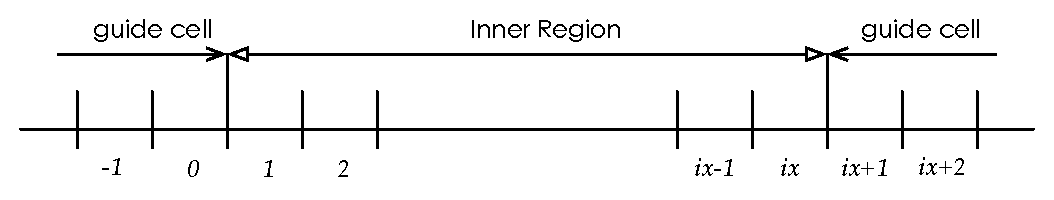
\includegraphics[width=12cm,clip]{index_domain.eps}
  \end{center}
  \caption{計算領域のインデクス}
  \label{fig:index_domain}
\end{figure}

\begin{figure}[htdp]
  \begin{center}
  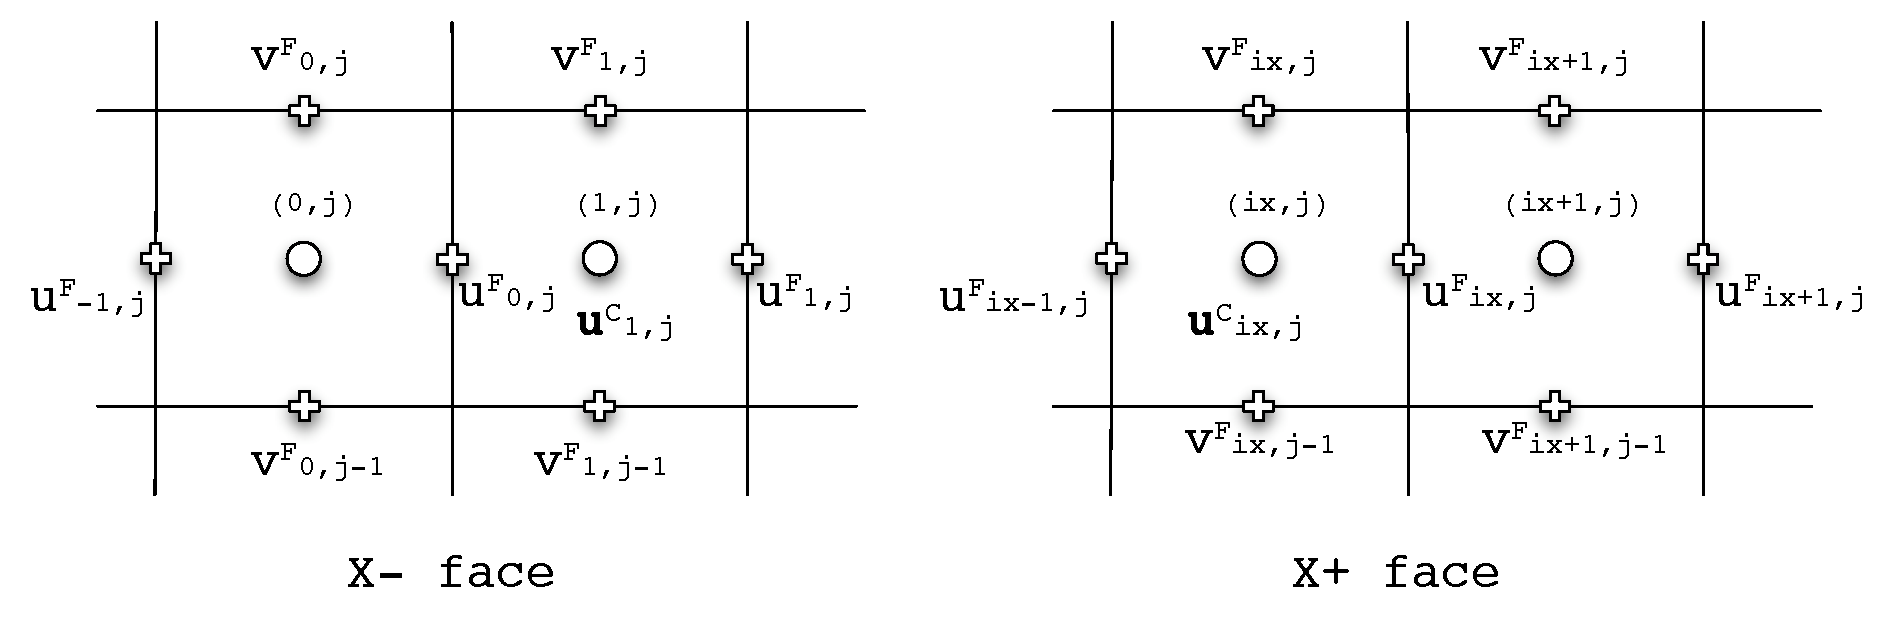
\includegraphics[width=14cm,clip]{index_cc.eps}
  \end{center}
  \caption{コロケート配置の変数のインデクス.基本変数($u_{\,i}^{\,C},\, p,\,\theta$)は全てセルセンタ位置に配置され,補助的な速度ベクトル$u_{\,i}^{\,F}$がスタガード位置に配置される.}
  \label{fig:index_cc}
\end{figure}


%
\subsection{流れの境界条件}
\label{sec:Boundary Conditions}

%
\subsubsection{壁面境界}
\label{sec:BC wall}

\begin{indentation}{3zw}{0zw}
\paragraph{外部境界面}
壁面境界条件は,外部境界条件の場合,XMLパラメータにより指定する.一方,計算領域内部に存在する壁面はセルIDにより指定され,その境界条件はEmbedded Boundary Condition Scheme\textbf{(\ref{sec:EBCS concept})}の仕組みを用いてスキームに組み込まれる.

外部境界は,壁面速度が時間的に変化する場合と固定の場合があり,指定する境界面の移動速度を与える.
ただし,壁面速度ベクトルは壁面と平行なスライド成分のみで,壁面と垂直な成分はゼロである点に注意する.

壁面境界は,Dirichlet型の速度境界条件を用いてセルフェイス位置の運動量流束を直接与える.外部境界では下記のようなXML入力パラメータで指定する.
次の例では,境界条件番号1にz軸に面直でy方向に7[m/s]で移動する壁の境界条件を指定している.

{\small
\begin{program}
<OuterBoundary>
  <Elem name="Basic_BCs">
    <Elem name="wall" id="1">
      <Param name="Normal_x"        dtype="REAL"   value="0.0" />
      <Param name="Normal_y"        dtype="REAL"   value="1.0" />
      <Param name="Normal_z"        dtype="REAL"   value="0.0" />
      <param name="Profile"         dtype="STRING" value="Harmonic" />
      <param name="Specified_Type"  dtype="STRING" value="Velocity" />
      <Param name="Specified_Value" dtype="REAL"   value="7.0" />
      <Param name="Frequency"       dtype="REAL"   value="2.0" />
      <Param name="Initial_Phase"   dtype="REAL"   value="0.0" />
      <Param name="Constant_Bias"   dtype="REAL"   value="0.0" />
    </Elem>
  </Elem>
</OuterBoundary>
\end{program}
}

\noindent 時間的に変化しない壁面境界の場合にはtype=constantを指定する.
時間変化を伴う速度指定はtype=harmonic\_oscillationを指定し,\textbf{式(\ref{eq:harmonic_v})}の形式の単振動\index{たんしんどう@単振動}の境界条件を周期や初期位相,切片(初期振幅)と供に与える\footnote{XMLの例ではコメントアウトされている.}.非定常の場合,振幅はvelocityで与えられる.

\begin{equation}
v \,{=}\, A \sin \left( 2 \mathrm{\pi} ft \,+\, \phi \right) \,+\, b
\label{eq:harmonic_v}
\end{equation}

ここで各パラメータは\textbf{表\ref{tbl:harmonic_table_v_obc}}に対応する.

\begin{table}[htdp]
\small
\caption{速度境界条件の単振動パラメータ}
\begin{center}
\begin{tabular}{lcll} \toprule
XMLキーワード & \textbf{式(\ref{eq:harmonic_v})}中の記号 & 説明 & 単位\\ \midrule
Amplitude & $A$ & 振幅 & $[m/s]$\\
Frequency & $f$ & 周波数 & $[Hz]$\\
Initial\_Phase & $\phi$ & 初期位相 & [rad]\\
Intercept & $b$ & 切片 & $[m/s]$\\ \bottomrule
\end{tabular}
\end{center}
\label{tbl:harmonic_table_v_obc}
\end{table}

計算領域内部の壁面境界条件は,EBCSの仕組みを用いてスキームに組み込まれ,セル界面の流束が指定する壁面速度から直接計算される.
したがって,計算する流体セルからみて,壁面方向に延びるステンシルのセルの値は参照されず不要である.
外部境界の場合には,可視化する場合の利便性を考慮し,出力時にのみガイドセルに値を書き出す.
この場合,境界面を中心に速度勾配一定として,速度成分を外挿する.

\begin{equation}
\left.
\begin{array}{llll}
\vspace{1mm}
\vspace{1mm} x-; & u_{\,0,\,j,\,k}    &=& 2\,u^{\,g} \,-\, u_{\,1,\,j,\,k}\\
\vspace{1mm}     & v_{\,0,\,j,\,k}    &=& 2\,v^{\,g} \,-\, v_{\,1,\,j,\,k}\\
\vspace{3mm}     & w_{\,0,\,j,\,k}    &=& 2\,w^{\,g} \,-\, w_{\,1,\,j,\,k}\\

\vspace{1mm} x+; & u_{\,ix+1,\,j,\,k} &=& 2\,u^{\,g} \,-\, u_{\,ix,\,j,\,k}\\
\vspace{1mm}     & v_{\,ix+1,\,j,\,k} &=& 2\,v^{\,g} \,-\, v_{\,ix,\,j,\,k}\\
\vspace{3mm}     & w_{\,ix+1,\,j,\,k} &=& 2\,w^{\,g} \,-\, w_{\,ix,\,j,\,k}\\

\vspace{1mm} y-; & u_{\,i,\,0,\,k}    &=& 2\,u^{\,g} \,-\, u_{\,i,\,1,\,k}\\
\vspace{1mm}     & v_{\,i,\,0,\,k}    &=& 2\,v^{\,g} \,-\, v_{\,i,\,1,\,k}\\
\vspace{3mm}     & w_{\,i,\,0,\,k}    &=& 2\,w^{\,g} \,-\, w_{\,i,\,1,\,k}\\

\vspace{1mm} y+; & u_{\,i,\,jx+1,\,k} &=& 2\,u^{\,g} \,-\, u_{\,i,\,jx,\,k}\\
\vspace{1mm}     & v_{\,i,\,jx+1,\,k} &=& 2\,v^{\,g} \,-\, v_{\,i,\,jx,\,k}\\
\vspace{3mm}     & w_{\,i,\,jx+1,\,k} &=& 2\,w^{\,g} \,-\, w_{\,i,\,jx,\,k}\\

\vspace{1mm} z-; & u_{\,i,\,j,\,0}    &=& 2\,u^{\,g} \,-\, u_{\,i,\,j,\,1}\\
\vspace{1mm}     & v_{\,i,\,j,\,0}    &=& 2\,v^{\,g} \,-\, v_{\,i,\,j,\,1}\\
\vspace{3mm}     & w_{\,i,\,j,\,0}    &=& 2\,w^{\,g} \,-\, w_{\,i,\,j,\,1}\\

\vspace{1mm} z-; & u_{\,i,\,j,\,kx+1} &=& 2\,u^{\,g} \,-\, u_{\,i,\,j,\,kx}\\
\vspace{1mm}     & v_{\,i,\,j,\,kx+1} &=& 2\,v^{\,g} \,-\, v_{\,i,\,j,\,kx}\\
\vspace{1mm}     & w_{\,i,\,j,\,kx+1} &=& 2\,w^{\,g} \,-\, w_{\,i,\,j,\,kx}\\
\end{array} \qquad \right \}
\label{eq:wall BC velocity}
\end{equation}


壁面境界に対する圧力の境界条件は,Navier-Stokes方程式からNeumann型の圧力境界条件が得られる.つまり,
\begin{equation}
{\frac{\partial p}{\partial x_{\,i}}}^{\,n+1} \,=\, - {\frac{\partial u_{\,i}}{\partial t}}^{\,n+1}
\,-\, \left( u_{\,j}-u_{\,j}^{\,g} \right) \frac{\partial u_{\,i}}{\partial x_{\,j}}
\,+\, \frac{1}{Re} \left( \frac{\partial^{\,2} u_{\,i}}{\partial x_{\,j}^{\,2}} \right)
\label{eq:prs BC from NS}
\end{equation}

\noindent 右辺の空間項は,\textbf{\ref{sec:Algorithm NS}}の各アルゴリズムに応じたタイムレベルで評価する.
レイノルズ数が小さい場合には粘性項の影響が無視できないが,
高レイノルズ数流れにおいては,粘性項の寄与が小さいと仮定し粘性項を省略する場合もある.
\begin{equation}
{\frac{\partial p}{\partial x_{\,i}}}^{\,n+1} \,=\, - {\frac{\partial u_{\,i}}{\partial t}}^{\,n+1}
\,-\, \left( u_{\,j}-u_{\,j}^{\,g} \right) \frac{\partial u_{\,i}}{\partial x_{\,j}}
\label{eq:prs BC from NS for High Re}
\end{equation}

\noindent \textbf{式(\ref{eq:prs BC from NS})},\textbf{(\ref{eq:prs BC from NS for High Re})}は,壁面の時間的・空間的な変化がない場合,

\begin{equation}
{\frac{\partial p}{\partial x_{\,i}}}^{\,n+1} \,=\, 
\frac{1}{Re} \left( \frac{\partial^{\,2} u_{\,i}}{\partial x_{\,i}^{\,2}} \right)
\label{eq:prs BC from NS for Low Re simple}
\end{equation}

\begin{equation}
{\frac{\partial p}{\partial x_{\,i}}}^{\,n+1} \,=\, 0
\label{eq:prs BC from NS for High Re simple}
\end{equation}


\noindent と簡単な形式になる.CBCソルバークラスでは,\textbf{(\ref{eq:prs BC from NS for High Re simple})}の壁面境界条件を用いている.
%\textbf{式(\ref{eq:prs BC from NS for Low Re simple})}
%全計算領域の壁面に対する境界条件として,高レイノルズ数型と低レイノルズ数型のどちらを用いるかをSteerセクションで指定しておく.
%次の例では,高レイノルズ数の場合の勾配ゼロを指定している.
%{ \small
%\begin{program}
%<Param name="Neumann_BCType_of_Pressure_on_solid_wall" dtype="string" value="grad_zero">
%\end{program}
%}

\vspace{5mm}
\paragraph{内部領域}
計算領域内部にある固体部分は,任意に現れる特徴があるので,その表面位置で粘着条件が課されるように対流項や粘性項のスキーム中で処理を行う.
セル界面が固体壁に接するかどうかは,セルの状態を表すビットフィールドからマスクを生成し,その情報を元に流束を計算する.
\end{indentation}

\pagebreak
%
\subsubsection{対称境界}
\label{sec:BC symmetric}

\begin{indentation}{3zw}{0zw}
外部境界にのみ用いられる境界条件で,指定する面が対称面であると仮定する.速度については,面直な成分のみ固体壁と同じで,残りはフリーとする.圧力は勾配がゼロとする.

\begin{equation}
\left.
\begin{array}{llll}
\vspace{1mm} x-; & u_{\,0,\,j,\,k}    &=& 2\,u^{\,g} \,-\, u_{\,1,\,j,\,k}\\
\vspace{1mm}     & v_{\,0,\,j,\,k}    &=& v_{\,1,\,j,\,k}\\
\vspace{1mm}     & w_{\,0,\,j,\,k}    &=& w_{\,1,\,j,\,k}\\
\vspace{3mm}     & p_{\,0,\,j,\,k}    &=& p_{\,1,\,j,\,k}\\

\vspace{1mm} x+; & u_{\,ix+1,\,j,\,k} &=& 2\,u^{\,g} \,-\, u_{\,ix,\,j,\,k}\\
\vspace{1mm}     & v_{\,ix+1,\,j,\,k} &=& v_{\,ix,\,j,\,k}\\
\vspace{1mm}     & w_{\,ix+1,\,j,\,k} &=& w_{\,ix,\,j,\,k}\\
\vspace{3mm}     & p_{\,ix+1,\,j,\,k} &=& p_{\,ix,\,j,\,k}\\

\vspace{1mm} y-; & u_{\,i,\,0,\,k}    &=& u_{\,i,\,1,\,k}\\
\vspace{1mm}     & v_{\,i,\,0,\,k}    &=& 2\,v^{\,g} \,-\, v_{\,i,\,1,\,k}\\
\vspace{1mm}     & w_{\,i,\,0,\,k}    &=& w_{\,i,\,1,\,k}\\
\vspace{3mm}     & p_{\,i,\,0,\,k}    &=& p_{\,i,\,1,\,k}\\

\vspace{1mm} y+; & u_{\,i,\,jx+1,\,k} &=& u_{\,i,\,jx,\,k}\\
\vspace{1mm}     & v_{\,i,\,jx+1,\,k} &=& 2\,v^{\,g} \,-\, v_{\,i,\,jx,\,k}\\
\vspace{1mm}     & w_{\,i,\,jx+1,\,k} &=& w_{\,i,\,jx,\,k}\\
\vspace{3mm}     & p_{\,i,\,jx+1,\,k} &=& p_{\,i,\,jx,\,k}\\

\vspace{1mm} z-; & u_{\,i,\,j,\,0}    &=& u_{\,i,\,j,\,1}\\
\vspace{1mm}     & v_{\,i,\,j,\,0}    &=& v_{\,i,\,j,\,1}\\
\vspace{1mm}     & w_{\,i,\,j,\,0}    &=& 2\,w^{\,g} \,-\, w_{\,i,\,j,\,1}\\
\vspace{3mm}     & p_{\,i,\,j,\,0}    &=& p_{\,i,\,j,\,1}\\

\vspace{1mm} z-; & u_{\,i,\,j,\,kx+1} &=& u_{\,i,\,j,\,kx}\\
\vspace{1mm}     & v_{\,i,\,j,\,kx+1} &=& v_{\,i,\,j,\,kx}\\
\vspace{1mm}     & w_{\,i,\,j,\,kx+1} &=& 2\,w^{\,g} \,-\, w_{\,i,\,j,\,kx}\\
\vspace{3mm}     & p_{\,i,\,j,\,kx+1} &=& p_{\,i,\,j,\,kx}\\
\end{array} \qquad \right \}
\label{eq:symmetric BC}
\end{equation}

次の例では,境界条件番号20に対称境界条件を設定する.
{ \small
\begin{program}
<OuterBoundary>
  <Elem name="Basic_BCs">
    <Elem name="symmetric" id="20"/>
  </Elem>
</OuterBoundary>
\end{program}
}
 
\end{indentation}


\pagebreak
%
\subsubsection{流出境界}
\label{sec:BC outflow}

\begin{indentation}{3zw}{0zw}
\paragraph{外部境界面}
流出境界を指定する場合には,流出方向は既知であり,外部境界面を指定することにより流出方向は決まる.
\textbf{図\ref{fig:outflow BC outer}}はX+方向の流出境界を示している.セル$(ix,\,j)$,セル$(ix+1,\,j)$ともに流体を指定する.
つまり,流出方向の外部領域は流体であるので,ガイドセル領域のIDをFace\_BCセクションで流体要素にしておく.
次の例では,id=20は流体要素である.

{\small
\begin{program}
<Elem name="Face_BC">
  <Elem comment="outflow" id="3" name="X_plus">
    <Param id="20" name="Guide_Cell_ID"/>
  </Elem>
</Elem>
\end{program}
}

\begin{figure}[htbp]
\begin{center}
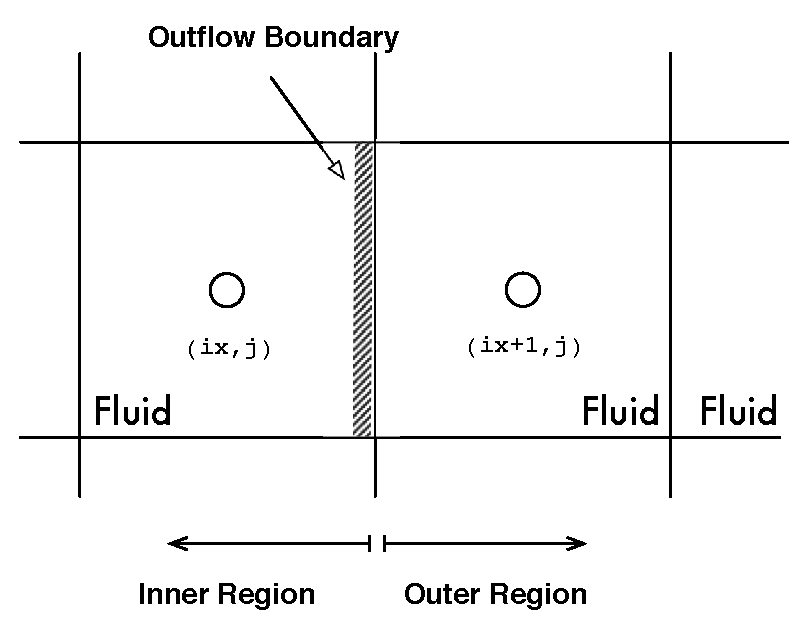
\includegraphics[width=8cm,clip]{outflowBC_outer.eps}
\end{center}
\caption{X+方向の流出境界の設定.}
\label{fig:outflow BC outer}
\end{figure}

次の例では,基本条件として3番に流出境界を登録している.

{\small
\begin{program}
<OuterBoundary>
  <Elem name="Basic_BCs">
    <Elem name="outflow" id="3">
      <Param name="velocity_type" dtype="STRING" value="minmax" />
    </Elem>
  </Elem>
</OuterBoundary>
\end{program}
}

流出境界面における流束は,境界面における流出速度から直接運動量を計算する.\textbf{図\ref{fig:outflow BC outer}}の例は$x$方向の流出面なので対流速度は$x$方向成分,非移流物理量を$\varphi$として,

\begin{equation}
{\left(\, \tilde{f}_i \,\right)}_{\,i+1/2,\,j,\,k} \,=\, {\left( u_{\,1}-u_{\,1}^{\,g} \right)}_{\,i+1/2,\,j,\,k} \,\varphi_{\,i,\,j,\,k}
\label{eq:outflow flux}
\end{equation}

\noindent 流出速度$u_{\,1}$は,セル$(\,i,\,j,\,k\,)$に対する連続の式から求める\footnote{BCvec\_cc.f90 $>$ vibc\_c\_out\_cf\_()}.流出速度は,コンポーネント毎の平均値もしくは最大値と最小値の算術平均を計算している.
流出速度の選び方として,流出断面の平均速度や最大値と最小値の算術平均などが提案されており,外部流や噴流のような無限空間の境界面の場合には,\textbf{式(\ref{eq:minmax outflow})}のMinMaxがよい近似値となる.
流出速度の指定は,Outflow\_Velocity タグにてaverage または minmaxを指定する.
Averageは有効セルの平均値をとる.有効セルは物体でブロックされていないセルである.
MinMaxは,境界面における流速の最大値と最小値の算術平均値を与える.

\begin{equation}
u_{ob} \,=\, \frac{1}{2} \{ max(u_{ob,j,k}) + min(u_{ob,j,k}) \}
\label{eq:minmax outflow}
\end{equation}

粘性項を評価する場合には,セルフェイス面での流出速度から勾配値が次式のように計算される.

\begin{equation}
{\left(\, \frac{\partial \varphi}{\partial x} \,\right)}_{\,i+1/2,\,j,\,k} \,=\, \frac{\varphi_{\,i+1/2,\,j,\,k}-\varphi_{\,i,\,j,\,k}}{h/2}
\label{eq:outflow grad1}
\end{equation}

\noindent コーディングでは格子幅を$h$としているので,勾配値が同じになるように流出速度を修正する\footnote{SetBC3D::modifyViscousEE(), SetBC3D::modifyViscousCN()を参照.\today 現在,この修正は行っていない.}.

\begin{equation}
\varphi_{\,i+1/2,\,j,\,k}^{\,\prime} \,=\, 2\, \varphi_{\,i+1/2,\,j,\,k} \,-\, \varphi_{\,i,\,j,\,k}
\label{eq:outflow grad2}
\end{equation}

\vspace{2mm}

実装としては,流出境界が指定された外部境界面にはBC Index bcv[]にid=31がエンコードされている.したがって,id=31の面に対して,セルセンターの変数に対して,流出境界を考慮した流束計算を行う.具体的には,流出速度が与えられるので,一次風上スキームを適用している\footnote{cbc\_pvec\_vobc(), MUSCLへ変更した方が良い}.


\paragraph{内部領域}
計算内部領域における流出境界は,\textbf{図\ref{fig:outflow BC inner}}のように,グレー部分,つまり$(i,\,j)\sim(i+1,\,j)$セル間の面が流出境界として指定されている.
境界面は,次のように対象となる面を2つのIDで挟むことにより指定する.
キーとなるIDは固体(この例ではid=20)を,def\_faceにid=210を指定し,$i+1/2$面を流出境界としている.
また,指定するid=20の属性は固体で,id=210の属性は流体であること.
加えて,固体セルは2層必要である\footnote{これはMUSCLスキームのステンシル長からの要請であるが,実装は未だupwind}.

{ \small
\begin{program}
<InnerBoundary>
  <Elem name="outflow" id="20" comment="outflow_sec_1">
    <Param name="def_face"      dtype="INT"    value="210" />
  </Elem>
</InnerBoundary>
\end{program}
}

\begin{figure}[htbp]
\begin{center}
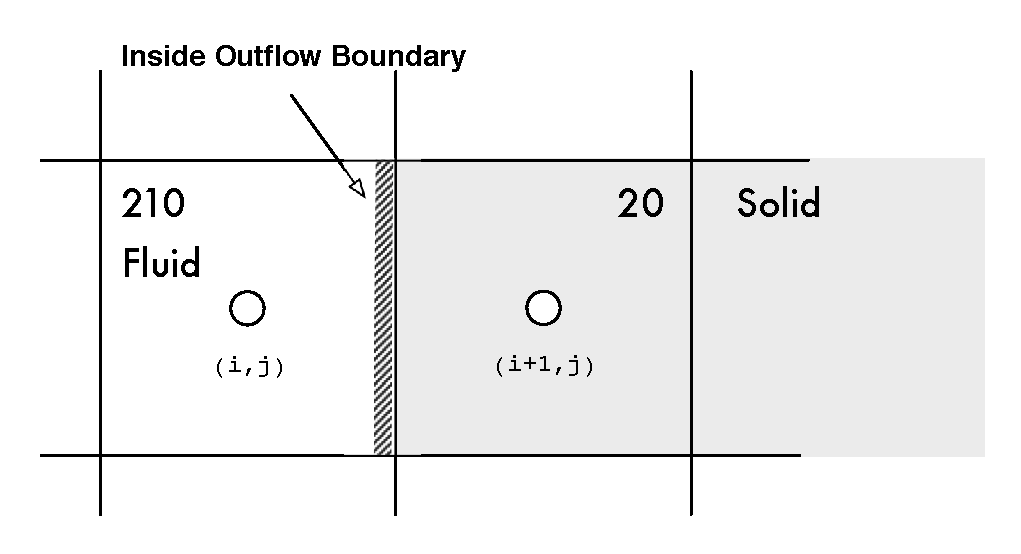
\includegraphics[width=9cm,clip]{outflowBC_inner.eps}
\end{center}
\caption{流出境界の設定.流出面の下流セルは固体とする.}
\label{fig:outflow BC inner}
\end{figure}

\noindent 流出速度の選び方として,経験上,内部流の場合にはAverageが流出速度のよい近似値を与える.
圧力境界として圧力勾配ゼロを指定している.

内部境界の流出fluxの計算は,現時点で一次風上となっているので,抜けにくい傾向があるかもしれない.


さて,Fractional Step法では,予測した疑似速度の発散に対して,連続の式を満足するように圧力場が収束していく.
そこで,Poisson方程式のソース項$\partial u_{\,i}^{\,*}/\partial x_{\,i}$に対して,次式のように流出境界面の指定速度が反映されるように修正している\footnote{SetBC3D::mod\_Psrc\_VBC(), cbc\_div\_ibc\_()を参照.}.

流出界面の流出速度には,次式の対流流出条件から時間進行した疑似速度ベクトルを用いる\footnote{SetBC3D::mod\_Pvec\_CF(), cbc\_vibc\_outflow\_cf\_()}.

\begin{equation}
{\frac{\partial u_{\,i}}{\partial t}}^{\,*} \,+\, {\left( u_{\,1} \right)}_{\,i+1/2} {\frac{\partial u_{\,i}}{\partial x}}^{\,n} \,=\, 0
\label{eq:outflow_cv}
\end{equation}


n+1ステップの速度を計算した後,流出セルフェイス面の速度を修正する.この修正されたセルフェイス速度を用いて,$div\,(\bm{u})^{\,n+1}$が評価され,収束判定に用いられる\footnote{収束判定のノルムの種類に$div\,(\boldmath $u$)^{\,n+1}$が指定されている場合.SetBC3D::modifyCFVelocity()を参照.}.

\begin{equation}
{\frac{\partial u_{\,i}}{\partial x_{\,i}}}^{\,*} \,=\, u_{\,i+1/2}^{\,n}-u_{\,i-1/2}^{\,*} + v_{\,j+1/2}^{\,*} - v_{\,j-1/2}^{\,*} + w_{\,k+1/2}^{\,*} - w_{\,k-1/2}^{\,*}
\label{eq:outflow modify poisson src}
\end{equation}

上記のように連続の式から逆に流出境界面速度を求める.しかしながらこの方法では,1つのセルに2つ以上の流出面は設定できない制限が生じる点に注意する.

%圧力の境界条件については,流出面で$\nabla p=0$を与える場合と,Dirichlet型$p=0$で与える場合を選択する.

\end{indentation}

\pagebreak
%
\hypertarget{tgt:inflow}{\subsubsection{速度指定境界}}
\label{sec:BC inflow}

速度指定境界は,流入境界として利用される.

\begin{indentation}{3zw}{0zw}

\paragraph{外部境界面}
流入境界を外部境界面に与える例を示す.

{ \small
\begin{program}
<OuterBoundary>
  <Elem id="2" name="Specified_Velocity">
    <Param dtype="REAL"   name="Normal_X"        value="1.0"/>
    <Param dtype="REAL"   name="Normal_Y"        value="0.0"/>
    <Param dtype="REAL"   name="Normal_Z"        value="0.0"/>
    <Param dtype="STRING" name="Specified_Type"  value="Velocity"/>
    <Param dtype="STRING" name="Profile"         value="Constant"/>
    <Param dtype="REAL"   name="Specified_Value" value="5.0"/>
  </Elem>
</OuterBoundary>
\end{program}
}

\textbf{図\ref{fig:inflow BC}}において,$w=i-1/2$面に速度$u_{\,1,\,\mathrm{in}}$を指定する場合を考える.セル$(i,\,j,\,k)$に対する流入条件なので$w$面の指定速度は$u_{\,1,\,\mathrm{in}}>0$になる.

\begin{equation}
{\left(\, \tilde{f}_i \,\right)}_{\,i-1/2,\,j,\,k} \,=\, u_{\,1,\,\mathrm{in}} \,\varphi_{\,\mathrm{in}}
\label{eq:inflow flux}
\end{equation}

\noindent 速度の流入境界の場合$\varphi$は次式となる.

\begin{equation}
\varphi_{\,\mathrm{in}} \,=\, u_{\,i,\,\mathrm{in}} \,+\,u_{\,i}^{\,g}
\label{eq:inflow flux}
\end{equation}

\begin{figure}[htbp]
\begin{center}
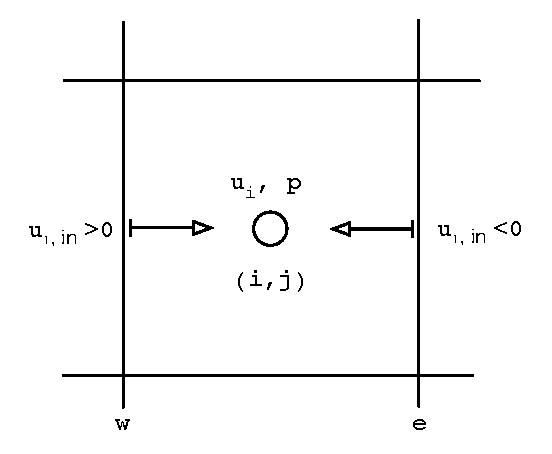
\includegraphics[width=5.5cm,clip]{inflowBC.eps}
\end{center}
\caption{速度指定境界.セル$\mathrm{(i,j)}$は流体セル,流入上流側の$\mathrm{(i\pm1,j)}$セルはガイドセル上で流体を指定する.}
\label{fig:inflow BC}
\end{figure}

速度指定境界条件は,流出条件と同様に流束型の境界条件として実装している\footnote{SetBC3D::mod\_Pvec\_Flux(), cbc\_pvec\_vobc\_()}.
指定部分で与えられた速度を用いて界面の流束を計算する.このとき,一次風上を用いているので,若干振動が残る.

圧力Poissonを解く場合の疑似速度の発散の修正は\verb|SetBC3D::mod_Psrc_VBC(), cbc_div_obc_vspec_()|で処理される.
また,セルフェイス速度は\verb|SetBC3D::mod\_Vec\_CF(), cbc\_vobc\_drchlt\_cf\_()|で計算する.

圧力の境界条件は,壁面境界条件と同様に,\textbf{式(\ref{eq:prs BC from NS})}のNavier-Stokes方程式からNeumann型の圧力境界条件が得られる.
流入境界における指定速度を$u_{\,i,\,in}$とすると,

\begin{equation}
{\left( \frac{\partial p}{\partial x_{\,i}}\right)}^{\,n+1}_{\,in} \,=\, - {\left( \frac{\partial u_{\,i}}{\partial t}\right)}^{\,n+1}_{\,in}
\,-\, \left( u_{\,j,\,in}-u_{\,j}^{\,g} \right) {\left( \frac{\partial u_{\,i}}{\partial x_{\,j}}\right)}_{\,in}
\,+\, \frac{1}{Re} {\left( \frac{\partial^{\,2} u_{\,i}}{\partial x_{\,j}^{\,2}} \right)}_{\,in}
\label{eq:prs inflow BC from NS}
\end{equation}

\noindent 高レイノルズ数流れにおいては,粘性項の寄与が小さいと仮定し粘性項を省略している.



\paragraph{内部領域}

指定方法として,Dirichlet型の速度境界条件を用いて,セルフェイス位置の運動量流束を直接与える.計算内部領域における流入境界のXML入力パラメータは下記のように指定する.

{\small
\begin{program}
<InnerBoundary> 
  <Elem name="specified_velocity" id="3" comment="inlet">
    <Param name="Normal_x"        dtype="REAL"   value="0.0" />
    <Param name="Normal_y"        dtype="REAL"   value="0.0" />
    <Param name="Normal_z"        dtype="REAL"   value="-1.0" />
    <Param name="def_face"        dtype="INT"    value="6" />
    <param name="Profile"         dtype="string" value="Harmonic" />
    <param name="Specified_Type"  dtype="string" value="Velocity" />
    <Param name="Specified_Value" dtype="REAL"   value="7.0" />
    <Param name="Frequency"       dtype="REAL"   value="2.0" />
    <Param name="Initial_Phase"   dtype="REAL"   value="0.0" />
    <Param name="Constant_Bias"   dtype="REAL"   value="0.0" />
    <Param name="Temperature"     dtype="REAL"   value="50.0" />
  </Elem>
</InnerBoundary>
\end{program}
}

\noindent 境界面の指定方法は流出境界と同様である.つまり,流入の上流側のセルには固体属性を与える.前述のXMLの指定の例では,id=6は流体セル,id=3は固体セルとなる.
ベクトルの指定は,法線成分とベクトルの大きさで与える.
時間的に変化しない場合にはtype=constantを指定する.
時間変化を伴う速度指定はtype=Harmonicを指定し,\textbf{式(\ref{eq:harmonic_v})}の形式の単振動\index{たんしんどう@単振動}の境界条件を周期や初期位相,切片(初期振幅)とともに与える.非定常の場合,振幅はvelocityで与えられる.
各パラメータは\textbf{表\ref{tbl:harmonic_table_v_obc}}に対応する.

\end{indentation}


\pagebreak
%
\subsubsection{周期境界}
\label{sec:BC periodic}

周期境界条件には,外部領域面に対する周期境界と計算内部領域に設定する部分的な周期境界条件を併用する条件の2種類を想定.

\begin{indentation}{3zw}{0zw}

\paragraph{外部領域面}

外部領域面に対する周期境界条件では,\textbf{図\ref{fig:index_domain}}において,Inner\,Regionの両端の境界が重なる状態を想定している.
外部領域面に対する周期境界条件には\textbf{表\ref{tbl:periodic mode}}に示す3つのモードが指定できる.

\begin{table}[htdp]
\caption{周期境界条件のモード}
\begin{center}
\small
\begin{tabular}{ll} \toprule
キーワード & モードの説明\\ \midrule
Simple\_Copy & 周期境界の両端で物理量をガイドセルにコピー.\\
Directional  & 圧力差を与える周期境界条件で,上流と下流の境界面を指定.\\
Driver       & 計算領域内で部分的な周期境界条件を設定.\\ \bottomrule
\end{tabular}
\end{center}
\label{tbl:periodic mode}
\end{table}

\begin{enumerate}
\item Simple\_Copyモード\\
周期境界条件面の両端で,単純に計算内部領域の値を他方のガイドセルにコピー.
\item Directionalモード\\
両端で圧力差を与える周期境界条件で,速度や温度についてはSimple\_Copyモードと同じだが,圧力は指定の圧力差を与える.上流側と下流側の設定が必要.
\item Driverモード\\
乱流計算などで発達したチャネル流を上流境界として与えるためのしくみで,内部境界条件との組み合わせで利用.Driverモードの説明は内部境界条件を参照.
\end{enumerate}


{\small
\begin{program}
<OuterBoundary>
  <Elem name="Basic_BCs">
    <Elem name="periodic" id="7" >
      <Param name="mode" dtype="string" value="Simple_Copy" />
    </Elem>
      
    <Elem name="periodic" id="8" >
      <Param name="mode"                dtype="string" value="Directional" />
      <Param name="flow_direction"      dtype="string" value="upstream" />
      <Param name="pressure_difference" dtype="REAL"   value="8.148e-3" />
    </Elem>
      
    <Elem name="periodic" id="9" >
      <Param name="mode"                dtype="string" value="Directional" />
      <Param name="flow_direction"      dtype="string" value="downstream" />
      <Param name="pressure_difference" dtype="REAL"   value="8.148e-3" />
    </Elem>
      
    <Elem name="periodic" id="10" >
      <Param name="mode"             dtype="string" value="driver" />
      <Param name="driver_direction" dtype="string" value="x_minus" />
    </Elem>
  </Elem>
</OuterBoundary>
\end{program}
}


Directionalモードでは,\textbf{表\ref{tbl:parameter dir. mode}}に示すパラメータが必要で,Pressure\_Differenceの値が,UpstreamとDownstreamで同じ値である必要がある.

\begin{table}[htdp]
\caption{Directionalモードに必要なパラメータ}
\begin{center}
\small
\begin{tabular}{ll} \toprule
必要なキーワード & パラメータの説明\\ \midrule
Pressure\_Difference & 両端にかける圧力差 $[Pa]$\\
Flow\_Direction & Upstream(上流面)または Downstream(下流面)\\
\bottomrule
\end{tabular}
\end{center}
\label{tbl:parameter dir. mode}
\end{table}


物理変数$\varphi$に対する周期境界条件は,Collocated変数配置\index{へんすうはいち@変数配置!コロケート@Collocated---}において,各方向について次式のように設定される.
適用の制限として,周期境界上には物体と他の境界条件を設定しないこと.

\begin{equation}
\begin{array}{ccc}
\left\{ \,\, \begin{array}{lll}
\varphi_{\,-2,\,j,\,k}   &=& \varphi_{\,ix-2,\,j,\,k}\\
\varphi_{\,-1,\,j,\,k}   &=& \varphi_{\,ix-1,\,j,\,k}\\
\varphi_{\,0,\,j,\,k}    &=& \varphi_{\,ix,\,j,\,k}\\
\varphi_{\,ix+1,\,j,\,k} &=& \varphi_{\,1,\,j,\,k}\\
\varphi_{\,ix+2,\,j,\,k} &=& \varphi_{\,2,\,j,\,k}
\end{array} \right. \quad
&
\left\{ \,\, \begin{array}{lll}
\varphi_{\,i,-2,\,k}     &=& \varphi_{\,i,\,jx-2,\,k}\\
\varphi_{\,i,-1,\,k}     &=& \varphi_{\,i,\,jx-1,\,k}\\
\varphi_{\,i,0,\,k}      &=& \varphi_{\,i,\,jx,\,k}\\
\varphi_{\,i,\,jx+1,\,k} &=& \varphi_{\,i,\,1,\,k}\\
\varphi_{\,i,\,jx+2,\,k} &=& \varphi_{\,i,\,2,\,k}
\end{array} \right. \quad
&
\left\{ \,\, \begin{array}{lll}
\varphi_{\,i,\,j,\,-2}   &=& \varphi_{\,i,\,j,\,kx-2}\\
\varphi_{\,i,\,j,\,-1}   &=& \varphi_{\,i,\,j,\,kx-1}\\
\varphi_{\,i,\,j,\,0}    &=& \varphi_{\,i,\,j,\,kx}\\
\varphi_{\,i,\,j,\,kx+1} &=& \varphi_{\,i,\,j,\,1}\\
\varphi_{\,i,\,j,\,kx+2} &=& \varphi_{\,i,\,j,\,2}
\end{array} \right.
\end{array}
\label{eq:periodic BC}
\end{equation}


\end{indentation}


\pagebreak
%
\subsubsection{遠方境界}
\label{sec:BC trc_free}

\begin{indentation}{3zw}{0zw}
トラクションフリー条件は,外部境界に対してのみ指定できる.
この境界条件は,計算対象の主領域から遠方の挙動を仮定した条件で,計算外部境界において流体の内部応力の法線方向成分がゼロである仮定を用いる.
この境界条件は,噴流のエントレインメントの効果などを考慮できる利点があるが,渦が流出するような境界には適用できない.
内部応力テンソルを$T_{\,ij}$, 計算外部境界の外向き法線を$n_{\,j}$とすると,

\begin{equation}
T_{\,ij} \,=\, - p \,\delta_{\,ij} \,+\,\nu \left( \frac{\partial u_{\,i}}{\partial x_{\,j}} \,+\, \frac{\partial u_{\,j}}{\partial x_{\,i}} \right)
\label{eq:Traction}
\end{equation}

\begin{equation}
T_{\,ij}\, n_{\,j} \,=\, 0
\label{eq:Tfree}
\end{equation}

\noindent 例えば,X軸の正負方向のトラクション成分を表す式は,次のように導出される.

\begin{equation}
\left[
\begin{array}{ccc}
T_{\,11} & T_{\,12} & T_{\,13}\\
T_{\,21} & T_{\,22} & T_{\,23}\\
T_{\,31} & T_{\,32} & T_{\,33}\\
\end{array} \right] \left[
\begin{array}{c}
\pm1\\
0\\
0\\
\end{array}
\right]
\,=\,
\pm \left[ 
\begin{array}{c}
T_{\,11}\\
T_{\,21}\\
T_{\,31}\\
\end{array} \right]
\,=\, \pm T_{\,i1} \,=\, 0
\label{eq:trc_eq}
\end{equation}

\noindent したがって,各外部境界面に対する解くべき式は次のように表せる.

\begin{equation}
\left .
\begin{array}{lll}
x & ; & T_{\,i1}\,=\,0 \\
y & ; & T_{\,i2}\,=\,0 \\
z & ; & T_{\,i3}\,=\,0  
\end{array}
\right \}
\label{eq:trc_eq2}
\end{equation}

\noindent 例えば,これからx方向の式を導くと,\textbf{式(\ref{eq:trc_eq3})}のようになる.

\begin{equation}
\left .
\begin{array}{l}
\vspace{2mm}
\displaystyle{ T_{\,11} \,=\, -p \,+\, 2 \nu \frac{\partial u_{\,1}}{\partial x_{\,1}} }\\
\vspace{2mm}
\displaystyle{ T_{\,21} \,=\, \frac{\partial u_{\,2}}{\partial x_{\,1}} + \frac{\partial u_{\,1}}{\partial x_{\,2}} }\\
\vspace{2mm}
\displaystyle{ T_{\,31} \,=\, \frac{\partial u_{\,3}}{\partial x_{\,1}} + \frac{\partial u_{\,1}}{\partial x_{\,3}} } 
\end{array}
\right \}
\label{eq:trc_eq3}
\end{equation}

\noindent \textbf{図\ref{fig:x-trc}}では,速度成分を$u,\,v,\,w$で表し,添え字で格子インデクスを表している.各方向の式を\textbf{式(\ref{eq:trc_cnd})}に示す.


\begin{figure}[htbp]
\begin{center}
\subfigure[X-方向のトラクションフリー条件.]{
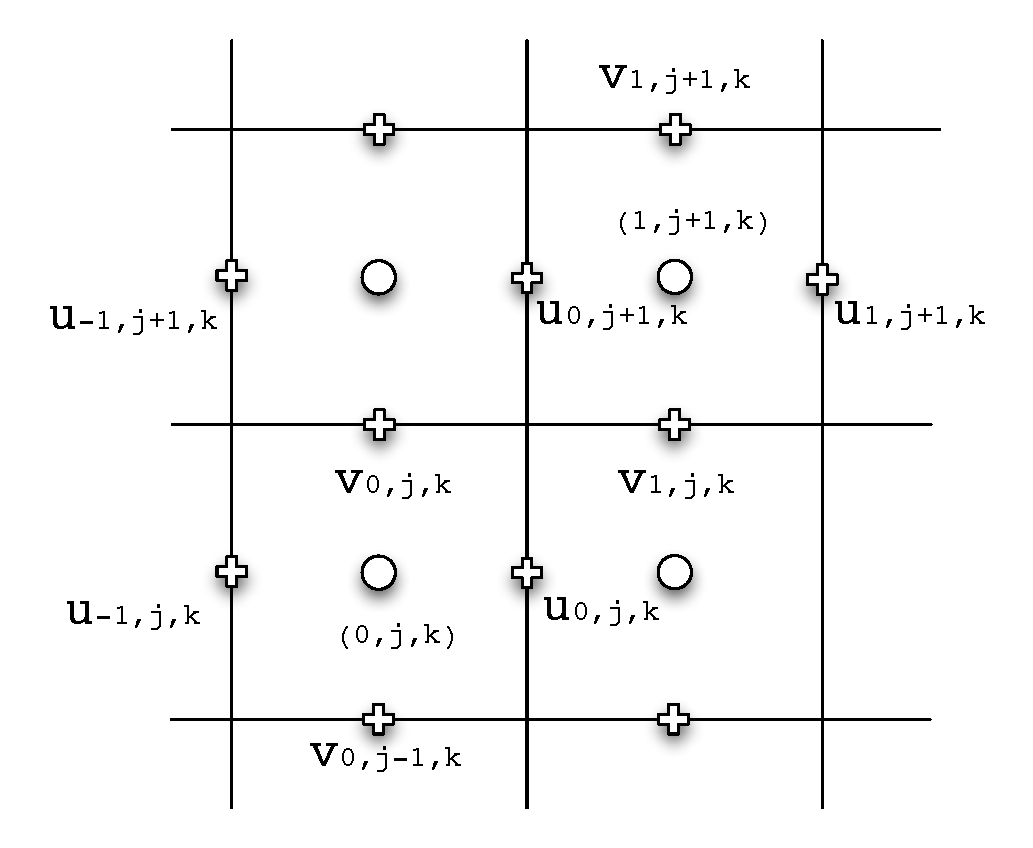
\includegraphics[height=6cm,clip]{T11.eps}
}~
\subfigure[X+方向のトラクションフリー条件.]{
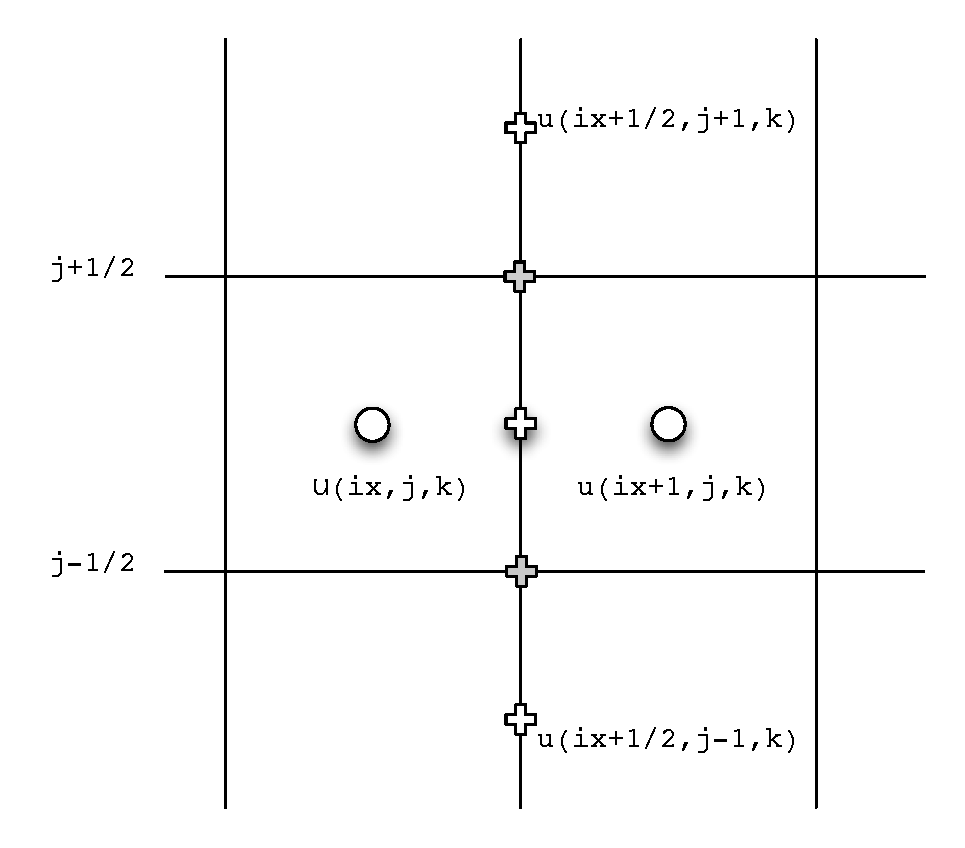
\includegraphics[height=6cm,clip]{T11+.eps}
}
\caption{外部境界のインデクス.} 
\label{fig:x-trc}
\end{center}
\end{figure}





\noindent 格子幅を$h$として$T_{\,21}$を外部境界面上で評価すると,
\begin{equation}
\left.
\begin{array}{l}
\vspace{1mm}
\displaystyle{ \frac{v_{\,1,\,j,\,k}-v_{\,0,\,j,\,k}}{h} \,+\, \frac{u_{\,1/2,\,j+1/2,\,k}-u_{\,1/2,\,j-1/2,\,k}}{h} \,\approx\, 
\frac{v_{\,1,\,j,\,k}-v_{\,0,\,j,\,k}}{h} \,+\, \frac{1}{2} \frac{u_{\,1/2,\,j+1,\,k}-u_{\,1/2,\,j-1,\,k}}{h} \,=\, 0 }\\
\vspace{1mm}
\displaystyle{ v_{\,0,\,j,\,k} \,=\, v_{\,1,\,j,\,k} \,+\, \frac{1}{2} \left( u_{\,1/2,\,j+1,\,k}-u_{\,1/2,\,j-1,\,k} \right) }\\
\end{array} \,\, \right\}
\label{eq:trc_T21}
\end{equation}

\noindent $u$はセルセンタ位置にあり,固体セルによる影響をマスク関数$\phi$で表すと,
\begin{equation}
\phi_{1/2,\,j,\,k} \,=\, \phi_{0,\,j,\,k} \times \phi_{1,\,j,\,k} \,=\,
\left\{
\begin{array}{ll}
0 & solid\\
1 & fluid\\
\end{array}
\right.
\end{equation}

\begin{equation}
u_{1/2,\,j\pm1,\,k} \,=\,(2u_{ref}-u_j)(1-\phi) + u_{j\pm1}\phi
\end{equation}

同様に,$T_{\,31}$から,
\begin{equation}
w_{\,0,\,j,\,k} \,=\, w_{\,1,\,j,\,k} \,+\, \frac{1}{2} \left( u_{\,1/2,\,j,\,k+1}-u_{\,1/2,\,j,\,k-1} \right)
\label{eq:trc_T31}
\end{equation}

\noindent $T_{\,11}$は圧力の遠方条件$p=0$(基準圧)を考慮して,
\begin{equation}
\frac{\partial u}{\partial x} \,=\, 0 \quad \mapsto \quad u_{\,0,\,j,\,k} \,=\, u_{\,1,\,j,\,k}
\label{eq:trc_T11}
\end{equation}

したがって,各方向の境界条件の式は以下のようになる.

\begin{equation}
\left.
\begin{array}{llll}
\vspace{1mm}
x-; & v_{0,\,j,\,k} & = & v_{1,\,j,\,k}\, +\, u_{0,\,j+1,\,k}\, -\, u_{0,\,j,\,k} \\
\vspace{1mm}
 & w_{0,\,j,\,k} & = & w_{1,\,j,\,k}\, +\, u_{0,\,j,\,k+1}\, -\, u_{0,\,j,\,k} \\
\vspace{4mm}
 & u_{-1,\,j,\,k} & = & u_{0,\,j,\,k}\,+\,v_{0,\,j,\,k}\,-\,v_{0,\,j-1,\,k}\,+\,w_{0,\,j,\,k}\,-\,w_{0,\,j,\,k-1}\\

\vspace{1mm}
x+; & v_{ix+1,\,j,\,k} & = & v_{ix,\,j,\,k}\, -\, u_{ix,\,j+1,\,k}\, +\, u_{ix,\,j,\,k} \\
\vspace{1mm}
 & w_{ix+1,\,j,\,k} & = & w_{ix,\,j,\,k}\, -\, u_{ix,\,j,\,k+1}\, +\, u_{ix,\,j,\,k} \\
\vspace{4mm}
 & u_{ix+1,\,j,\,k} & = & u_{ix,\,j,\,k}\,-\,v_{ix+1,\,j,\,k}\,+\,v_{ix+1,\,j-1,\,k}\,-\,w_{ix+1,\,j,\,k}\,+\,w_{ix+1,\,j,\,k-1}\\

\vspace{1mm}
y-; & u_{i,\,0,\,k} & = & u_{i,\,1,\,k}\, +\, v_{i+1,\,0,\,k}\, -\, v_{i,\,0,\,k} \\
\vspace{1mm}
 & w_{i,\,0,\,k} & = & w_{i,\,1,\,k}\, +\, v_{i,\,0,\,k+1}\, -\, v_{i,\,0,\,k} \\
\vspace{4mm}
 & v_{i,\,-1,\,k} & = & v_{i,\,0,\,k}\,+\,u_{i,\,0,\,k}\,-\,u_{i-1,\,0,\,k}\,+\,w_{i,\,0,\,k}\,-\,w_{i,\,0,\,k-1}\\

\vspace{1mm}
y+; & u_{i,\,jx+1,\,k} & = & u_{i,\,jx,\,k}\, -\, v_{i+1,\,jx,\,k}\, +\, v_{i,\,jx,\,k} \\
\vspace{1mm}
 & w_{i,\,jx+1,\,k} & = & w_{i,\,jx,\,k}\, -\, v_{i,\,jx,\,k+1}\, +\, v_{i,\,jx,\,k} \\
\vspace{4mm}
 & v_{i,\,jx+1,\,k} & = & v_{i,\,jx,\,k}\,-\,u_{i,\,jx+1,\,k}\,+\,u_{i-1,\,jx+1,\,k}\,- \,w_{i,\,jx+1,\,k}\,+\, w_{i,\,jx+1,\,k-1}\\

\vspace{1mm}
z-; & u_{i,\,j,\,0} & = & u_{i,\,j,\,1}\, +\, w_{i+1,\,j,\,0}\, -\, w_{i,\,j,\,0} \\
\vspace{1mm}
 & v_{i,\,j,\,0} & = & v_{i,\,j,\,1}\, +\, w_{i,\,j+1,\,0}\, -\, w_{i,\,j,\,0} \\
\vspace{4mm}
 & w_{i,\,j,\,-1} & = & w_{i,\,j,\,0}\,+\,u_{i,\,j,\,0}\,-\,u_{i-1,\,j,\,0}\,+\,v_{i,\,j,\,0}\,-\,v_{i,\,j-1,\,0}\\

\vspace{1mm}
z-; & u_{i,\,j,\,kx+1} & = & u_{i,\,j,\,kx}\, -\, w_{i+1,\,j,\,kx}\, +\, w_{i,\,j,\,kx} \\
\vspace{1mm}
 & v_{i,\,j,\,kx+1} & = & v_{i,\,j,\,kx}\, -\, w_{i,\,j+1,\,kx}\, +\, w_{i,\,j,\,kx} \\
\vspace{4mm}
 & w_{i,\,j,\,kx+1} & = & w_{i,\,j,\,kx}\,-\,u_{i,\,j,\,kx+1}\,+\,u_{i-1,\,j,\,kx+1}\,-\, v_{i,\,j,\,kx+1}\,+\, v_{i,\,j-1,\,kx+1}
\end{array}
\right \}
\label{eq:trc_cnd}
\end{equation}


実装では,壁面上の速度成分はマスク関数でマスクし,速度をゼロにしている.

j=jxの場合に,$u_{0,\,jx+1,\,k}$の値を参照するので,境界条件処理で値を代入しておく必要がある.

次の例では,遠方圧力に$p=0$[Pa\_g]\footnote{ゲージ圧,Steer $>$ Unit $>$ PressureでGaugeを指定しておく.}を指定した境界条件ID=4に遠方境界条件を設定する.熱流れの場合には,遠方場における温度を指定.
{ \small
\begin{program}
<OuterBoundary>
  <Elem name="Basic_BCs">
    <Elem name="traction_free" id="4">
      <Param name="Ambient_Temperature" dtype="REAL" value="25.0" />
    </Elem>
  </Elem>
</OuterBoundary>
\end{program}
}
\end{indentation}


\pagebreak
%
\subsubsection{流入出境界}
\label{sec:BC in_out}

\begin{indentation}{3zw}{0zw}
振動流のための特殊な境界条件である.指定された外部境界面において,境界流速の符号に応じて流出と遠方条件を切り替える.
境界流速には境界面の平均流速を用いる.

下記の例では,流出境界条件に切り替わった場合の対流流出速度のパラメータをMinmaxに指定.

{\small
\begin{program}
<OuterBoundary>
  <Elem name="in_out" id="5">
    <Param name="velocity_type" dtype="STRING" value="minmax" />
    <Param name="Ambient_Temperature" dtype="REAL" value="25.0" />
  </Elem>
</OuterBoundary>
\end{program}
}

熱流れの場合には,流入時に対応する温度を指定.

\end{indentation}

\pagebreak
%
\subsection{静止座標系と移動座標系の場合の境界条件}
\label{sec:moving_grid}
外部流を考える.
\textbf{図\ref{fig:reference_frame}}(a)の静止座標系\index{ざひょうけい@座標系!せいし@静止---}と{図\ref{fig:reference_frame}}(b)の移動座標系\index{ざひょうけい@座標系!いどう@移動---}のように異なる座標系で物体まわりの流れを計算する場合,境界条件の与え方が異なる.
静止座標系は風洞実験に相当し,静止した対象物に対して風をあてる.テストセクション(この場合は計算領域)から出ていく流れが流出風に相当する.
一方,移動座標系では対象物に固定した計算格子が対象物とともに静止流体中を移動する.この場合は,計算領域そのものと内部の格子が物体とともに動く.
一定速度$V$で動いている座標系の添え字を${}_M$とし,静止した座標系の添え字を${}_S$とする.
いま,静止座標系で観測される流体の速度を$u_{S}$と表すと,同じ速度は移動座標系では$u_{M}-V$のように観測される.
つまり,
\begin{equation}
u_{S} \, = \, u_{M}-V
\label{eq:galilei}
\end{equation}
両者は\textbf{式(\ref{eq:galilei})}のガリレイ変換\index{がりれいへんかん@ガリレイ変換}に対して不変である.

\begin{figure}[htbp]
\begin{center}
\subfigure[静止座標系]{
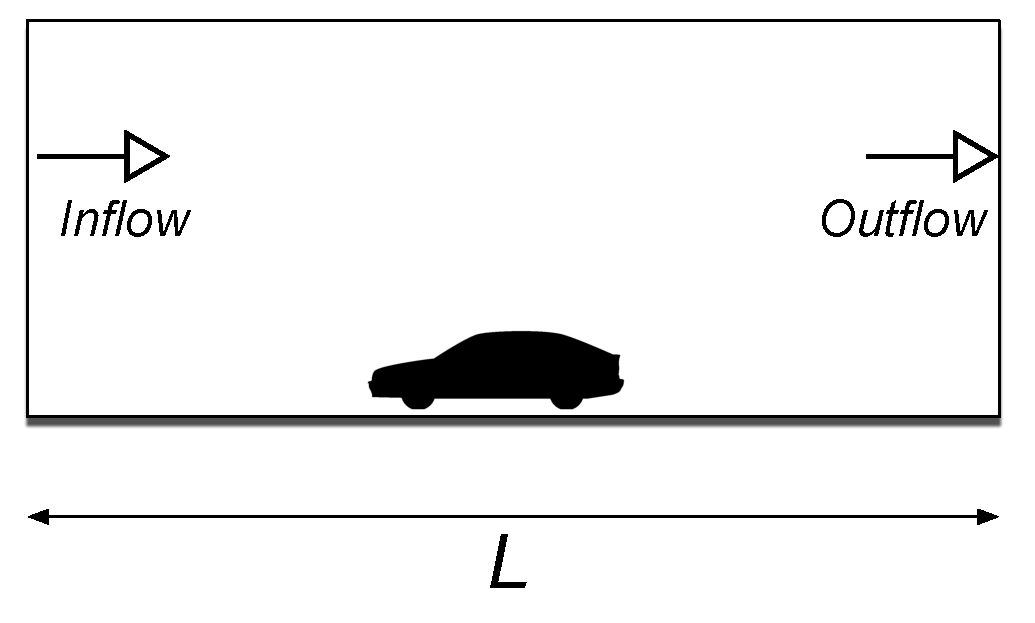
\includegraphics[width=8cm,clip]{stationary.eps}
}
~
\subfigure[移動座標系]{
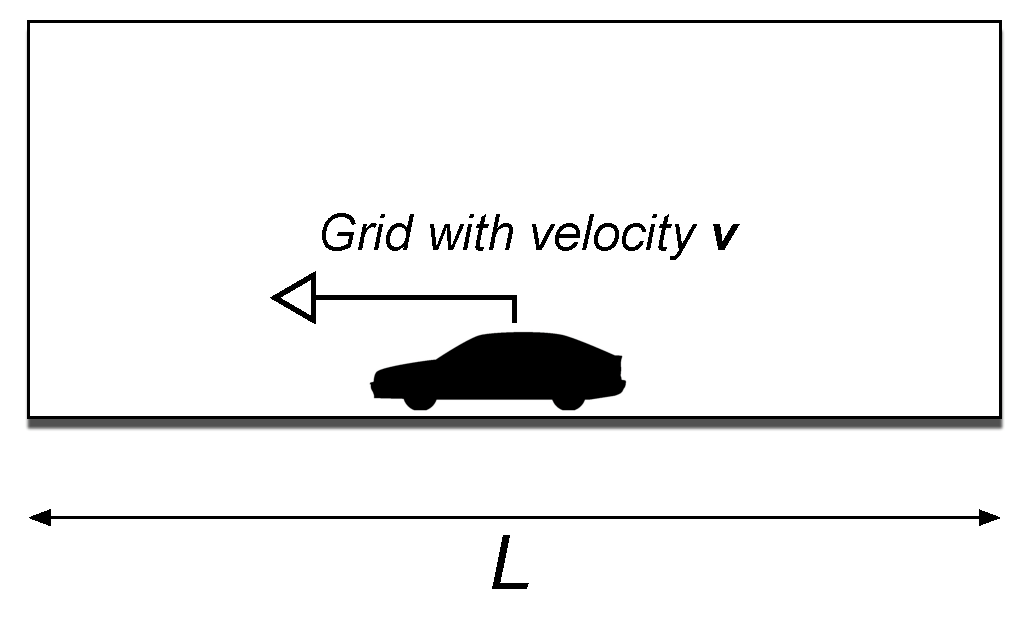
\includegraphics[width=8cm,clip]{moving.eps}
}
\caption{静止座標系と移動座標系の観測点の違い} 
\label{fig:reference_frame}
\end{center}
\end{figure}

静止座標系において\textbf{図\ref{fig:reference_frame}}(a)のような境界条件を与える場合,流入部では$u_{0}$を与える.
一方,移動座標系では静止流体の条件,つまり$u=0,\,p=0$を想定し,格子速度$V=-u_{0}$を与えると両者は等価になる.

移動座標系の場合注意を要するのが,物体と地面の境界条件である.物体は移動しているので格子速度と同じである.
一方,地面は静止している地面と動いている地面の二通りが考えられる.
前者は風洞実験で固定地面板に相当し,後者はムービングベルトに相当する.
ムービングベルトの場合には物体と格子速度だけ相対速度をもっている.
したがって,

\begin{equation}
u_{ground}\,=\,
\begin{cases}
\, -u_{0} & \quad (Stationary\,ground)\\
\, 0 & \quad (Moving\,ground)\\
\end{cases}
\label{eq:relative velocity wall}
\end{equation}

移動格子の移動速度はReference\_Frameセクションで与える.




%%%%%
\begin{comment}
%
%
\paragraph{Direct\_Forcing}
\begin{indentation}{3zw}{0zw}
%Direct\_Forcingによる指定は,速度定義点により記述するカテゴリが異なる.
Immersed Boundary Methodの定式化に従い,定義点において速度を強制する.
次の例では,ID=2のセルのスタガード位置の速度定義点に指定した法線と大きさをもつ速度を強制する.
モニター量はない.

{ \small
\begin{program}
<Elem name="Vec_Face" id="1">
  <Elem name="direct_forcing" id="2" comment="f1">
    <Param name="Norm_x"      dtype="REAL"   value="1.0" />
    <Param name="Norm_y"      dtype="REAL"   value="0.0" />
    <Param name="Norm_z"      dtype="REAL"   value="0.5" />
    <Param name="velocity"    dtype="REAL"   value="0.5" />
  </Elem>
</Elem>
\end{program}
}

%%%

次の例は,セルセンタ位置での指定を示す.
{ \small
\begin{program}
<Elem name="Vec_Center" id="1">
  <Elem name="direct_forcing" id="2" comment="f1">
    <Param name="Norm_x"      dtype="REAL"   value="1.0" />
    <Param name="Norm_y"      dtype="REAL"   value="0.0" />
    <Param name="Norm_z"      dtype="REAL"   value="0.5" />
    <Param name="velocity"    dtype="REAL"   value="0.5" />
  </Elem>
</Elem>
\end{program}
}

%%%
\end{indentation}

\end{comment}
%%%%%


\pagebreak
%
\subsection{外力項を用いた境界条件}

\subsubsection{圧力損失・利得を伴う境界条件}
熱交換器やファンなどの圧力損失\index{あつりょくそんしつ@圧力損失}・利得をモデル化した境界条件について説明する.
熱交換器は,圧力損失を生じる多孔質物体で,流出方向が法線で与えられる.圧力損失は通過流量(流速)と圧力損失量の関係式が与えられるものとする.
一方,ファンは流量と圧力利得が関係式として与えられる.ファンの場合には旋回成分などもあるが,ここでは軸流方向のみを考える.
このような流体部品のモデル指定は,セルボリュームに作用する内部境界条件として指定し,コンポーネントを用いて実装する.
具体的には,\textbf{式(\ref{eq:ploss_NS})}の外力項$F_{i}$として実装する.$\beta$はセル内部におけるコンポーネントの体積占有率\index{せんゆうりつ@占有率}(Volume Fraction; VF)\index{Volume Fraction}である.
外力項として,\textbf{表\ref{tbl:ploss_model}}のようなモデルが実装されている.

この境界条件に対応する指定部の平均速度・流量や圧力損失量がhistory\_compo.logにモニタ量として書き出される.

\begin{table}[htdp]
\caption{セルボリュームに作用する内部境界条件}
\begin{center}
\small
\begin{tabular}{lll} \toprule
XMLキーワード & 境界条件モデル & モニター量\\ \midrule
%Fan & ファンモデル & \\ 
Pressure\_Loss & 圧力損失モデル & 通過風速,圧力損失量\\ 
%Darcy & 多孔質体に対するDarcyモデル & \\ 
\bottomrule
\end{tabular}
\end{center}
\label{tbl:ploss_model}
\end{table}

\begin{equation}
{\frac{\partial{u}_{i}}{\partial{t}}}^{{n}{+}{1}}{+}\,\frac{\partial}{\partial{x}_{j}}\left({{u}_{i}{u}_{j}}\right)
\,{=}\,
{-}{\frac{\partial{p}}{\partial{x}_{i}}}^{{n}{+}{1}}{+}\,{(}{1}{-}\mathrm{\beta}{)}\frac{\partial{\mathrm{\tau}}_{ij}}{\partial{x}_{j}}\,{+}\,\beta {F_{i}}^{n+1}
\label{eq:ploss_NS}
\end{equation}

%
\paragraph{Pressure\_Loss}
\begin{indentation}{3zw}{0zw}
圧力損失モデルは,膜や熱交換器などのモデリングとして利用され,\textbf{式(\ref{eq:ploss_NS})}に\textbf{式(\ref{eq:ploss_force})}の実験式を適用する.
\begin{equation}
{F}_{i}
\,{=}\,
-sgn \left( u_{i} \right) {\left( \frac{\Delta p}{\Delta r} \right)}^{R} {n_{i}}^{R}
\label{eq:ploss_force}
\end{equation}

\noindent ここで,${}^{R}$は圧力損失部を表し,$\Delta p,\,\Delta r,\,n_{i}$はそれぞれ圧力損失量,圧力損失部の厚さ,法線方向を表す.圧力損失部の通過ベクトルとは逆方向に圧力損失が発生するモデルとなっている.ただし,\textbf{表\ref{tbl:ploss_table_ibc}}で指定するパラメータvectorがdirectionalでない場合には,速度ベクトルは圧力損失部の流出方向には揃わない.単に,圧力損失が計算された速度ベクトルと逆向きに作用するモデルとなる.

圧力損失パラメータは,圧力損失部の試験結果により,\textbf{図\ref{fig:ploss}}に示すような実験値が得られる.
$\Delta p-V$の性能線図を$[mmAq - m/s]$を単位とした場合のパラメータの取得について示す.
圧力損失部の圧力損失は大抵二次多項式で近似できる.
\textbf{図\ref{fig:ploss}}のグラフの読みからカーブフィットを行い,\textbf{式(\ref{eq:dp-v})}に対応する数値$c_{1}$ -- $c_{4}$, $u_{threshold}$を得る.ダッシュは有次元を表す.
このとき,圧力損失ヘッドの単位に応じて,パラメータは無次元量に変換している.

\begin{equation}
{h}^{\prime}
\,{=}\,
\begin{cases}
\, c_{1} {u^{\prime}}^{2}\,+\,c_{2}u^{\prime}\,+\,c_{3} & \quad (u^{\prime} \geqq u^{\prime}_{threshold})\\
\, c_{4} {u^{\prime}}^{2} & \quad (u^{\prime}<u^{\prime}_{threshold})\\
\end{cases} \quad [mm]
\label{eq:dp-v}
\end{equation}

\vspace{5mm}

\begin{figure}[htdp]
  \begin{minipage}{.47\textwidth}
    \begin{center}
  	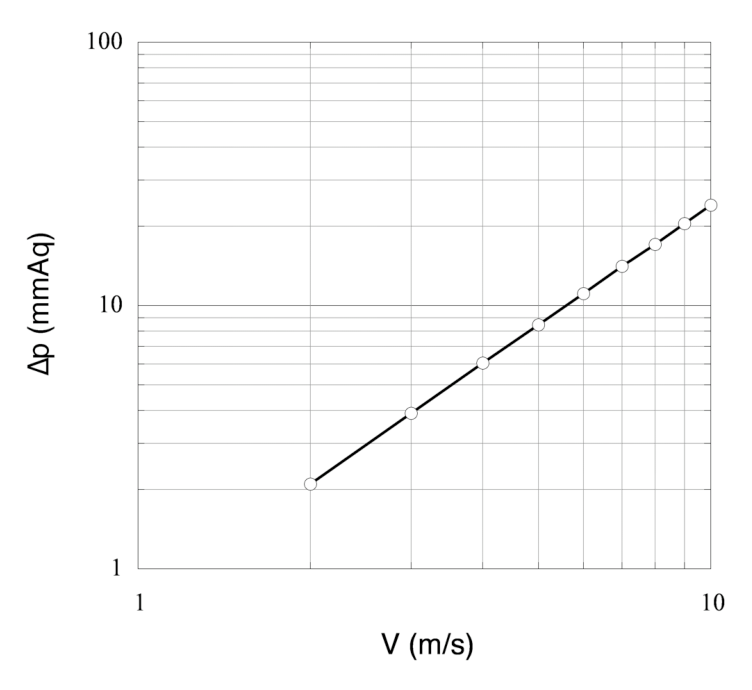
\includegraphics[width=6.5cm,clip]{ploss.eps}
  	\end{center}
  	\caption{$\Delta p-V$性能線図(対数表示)}
  	\label{fig:ploss}
  \end{minipage} \hfill
  \begin{minipage}{.47\textwidth}
    \begin{center}
    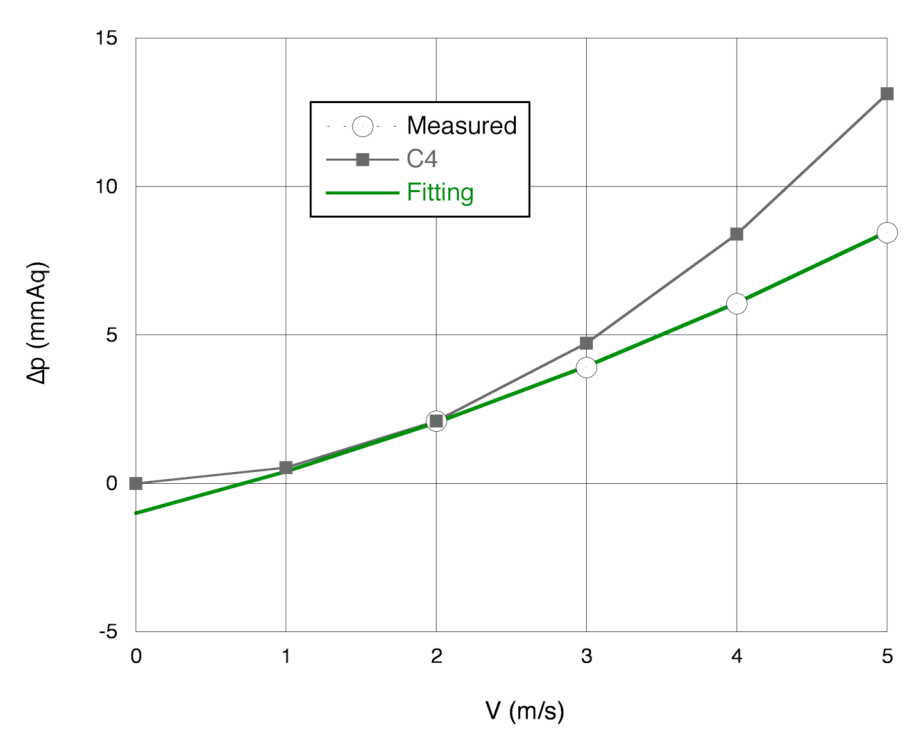
\includegraphics[width=7.5cm,clip]{rad_para.eps}
    \caption{パラメータの取得(\textbf{図\ref{fig:ploss}}と同じものを線形表示)}
    \label{fig:get_para}
    \end{center}
  \end{minipage}
\end{figure}

\textbf{図\ref{fig:get_para}}に計算パラメータの取得方法を示す.一般に,低速域のデータは得られない場合が多い.図では,○が測定結果を示し2$[m/s]$より低速域のデータはない.そこで,測定値を元にカーブフィッティングを行い(図中の緑色の曲線),算出された係数$c_{1}=0.12321,\,c_{2}=1.2806,\,c_{3}=-1.0074\quad(2-10\,[m/s])$を計算パラメータとする.この場合,$h'$切片がマイナスになるため,熱交換機の通過速度がゼロに近い場合に急にマイナスの圧力損失(つまり圧力利得)が発生し,実際の現象とは異なり計算上好ましくない.そこで\textbf{式(\ref{eq:dp-v})}に示すようにある閾値で曲線を切り替える.ここでは,測定された最小速度$u_{threshold}=2\,[m/s]$を閾値として,図中のC4のカーブ$c_{4}=0.525\quad(0-2\,[m/s])$で切り替える.圧力損失部厚さは実務での観点から単位を$[mm]$で指定するので,注意のこと.詳細については,\ref{sec:external force method}を参照.

次の例では,境界条件番号50に圧力損失条件を設定する.
ここで各パラメータは\textbf{表\ref{tbl:ploss_table_ibc}}に対応する.
{ \small
\begin{program}
<Elem name="Pressure_Loss" id="50" comment="radiator">
  <Param name="Normal_x"    dtype="REAL"   value="5.0" />
  <Param name="Normal_y"    dtype="REAL"   value="0.0" />
  <Param name="Normal_z"    dtype="REAL"   value="-1.0" />
  <Param name="c1"          dtype="REAL"   value="2.0" />
  <Param name="c2"          dtype="REAL"   value="10.0" />
  <Param name="c3"          dtype="REAL"   value="0.0" />
  <Param name="c4"          dtype="REAL"   value="0.0" />
  <Param name="u_threshold" dtype="REAL"   value="0.5" />
  <Param name="thickness"   dtype="REAL"   value="0.05" />
  <Param name="unit"        dtype="STRING" value="mmAq" />
  <Param name="vector"      dtype="STRING" value="directional" />
<\Elem>
\end{program}
}

\begin{table}[htdp]
\caption{圧力損失モデルのパラメータ}
\begin{center}
\small
\begin{tabular}{lll} \toprule
XMLキーワード & パラメータの説明\\ \midrule
Normal\_x & 圧力損失部の法線ベクトルのx方向成分\quad 法線は単位ベクトル\\
Normal\_y & 圧力損失部の法線ベクトルのy方向成分\quad 法線は単位ベクトル\\
Normal\_z & 圧力損失部の法線ベクトルのz方向成分\quad 法線は単位ベクトル\\
c1 & 圧力損失部の圧力損失係数\,c1\quad $[mmAq\,|\,mmHg\,|\,Pa]$\\
c2 & 圧力損失部の圧力損失係数\,c2\quad $[mmAq\,|\,mmHg\,|\,Pa]$\\
c3 & 圧力損失部の圧力損失係数\,c3\quad $[mmAq\,|\,mmHg\,|\,Pa]$\\
c4 & 圧力損失部の圧力損失係数\,c4\quad $[mmAq\,|\,mmHg\,|\,Pa]$\\
u\_threshold & 圧力損失カーブの切り替え速度 $u_{threshold}$ $[m/s]$\\
thickness & 圧力損失部の厚さ\quad $[mm]$\\
unit & 圧力損失$\Delta p-V$線図のヘッドの単位\quad [$mmAq\,|\,mmHg\,|\,Pa\,|\,Non-Dimension]$ \footnotemark[7]\\
vector & 速度ベクトルの法線方向への強制\quad $[Directional \,|\, Non-Directional]$\\  \bottomrule
\end{tabular}
\end{center}
\label{tbl:ploss_table_ibc}
\end{table}
\footnotetext[7]{mmAqは水(300K, p=101.325kPa)996.62 $[kg/m^3]$,mmHgは水銀(300K)13538 $[kg/m^3]$をプログラム中でハードコード.}
\end{indentation}






%%%%
\begin{comment}
\paragraph{Fan}
\begin{indentation}{3zw}{0zw}
Fanモデル...
\end{indentation}

%
\paragraph{Darcy model}
\label{Darcy model param}
\begin{indentation}{3zw}{0zw}

\ref{sec:porous model}で説明したDarcyモデルでは,等方と非等方モデルが利用できる.透過率パラメータは,\textbf{表\ref{tbl:permeability parameter}}に示すように各主軸方向毎に与える.等方モデルの場合には,各方向のパラメータを同じ値にする.

{ \small
\begin{program}
<Elem name="Forcing_Volume" id="1">
  <Elem name="Darcy" id="50" comment="porous">
    <Param name="permeability_x"  dtype="REAL" value="2.0" />
    <Param name="permeability_y"  dtype="REAL" value="3.0" />
    <Param name="permeability_z"  dtype="REAL" value="4.0" />
  <\Elem>
<\Elem>
\end{program}
}

\begin{table}[htdp]
\caption{Darcyモデルのパラメータ}
\begin{center}
\small
\begin{tabular}{ll} \toprule
XMLキーワード & パラメータの説明\\ \midrule
permeability\_x & x方向の透過率 $[m^2]$\\
permeability\_y & y方向の透過率 $[m^2]$\\
permeability\_z & z方向の透過率 $[m^2]$\\ \bottomrule
\end{tabular}
\end{center}
\label{tbl:permeability parameter}
\end{table}

\end{indentation}

\end{comment}
%%%%

%
\section{熱解析の境界条件}
\label{sec:thermal_condition}
非圧縮性流体近似されたエネルギー式,つまりパッシブスカラー型の温度輸送方程式について,温度の境界条件を説明する.流れの境界条件と同様に,まず,外部境界条件を\ref{sec:heat_ext_bc}で説明し,その後内部境界条件を\ref{sec:heat_int_bc}で説明する.内部境界条件には熱交換機での利用を想定した放熱境界条件を含む.

%
\subsection{外部境界条件の指定}
\label{sec:heat_ext_bc}
熱の外部境界条件は,\ref{sec:heat_boundary}で詳しく述べているが,断熱条件はマスク\index{マスク}により温度勾配ゼロの条件が直接反復式中に取り込まれる.また,熱伝導条件は拡散項で表現され多媒質の場合に物性値依存で熱移動が計算される.これらの2つ以外の境界条件は明示的に指定する.

\textbf{表\ref{tbl:temperature_obc}}に示す熱の外部境界条件について例示する.熱の境界条件は,全て有次元でパラメータを与える.

%
\paragraph{Dirichlet}
\begin{indentation}{3zw}{0zw}
指定面のガイドセルに指定温度を与える.
次の例では,境界条件番号40として,20.0 [${}^\circ \mathrm{C}$ or K]のDirichlet境界条件を設定する.温度の単位はUnit\_Temperatureに従う.
{ \small
\begin{program}
<Param name="dirichlet" dtype="REAL" value="20.0" id="40"/>
\end{program}
}
\end{indentation}

%%%
\begin{comment}
\paragraph{HeatFlux}
\begin{indentation}{3zw}{0zw}
指定面に熱流束を指定する.
次の例では,境界条件番号40として,熱流束境界条件を設定する.
{ \small
\begin{program}
<Param name="HeatFlux" dtype="REAL" value="" id="40"/>
\end{program}
}
\end{indentation}
\end{comment}
%%%

%
\paragraph{Insulation}
\begin{indentation}{3zw}{0zw}
指定面で断熱条件を指定する.
断熱条件の実効的な実装は,内部境界条件の断熱指定によるので,ここでは単にガイドセルへの値のコピーを行っているだけである.
次の例では,境界条件番号30に断熱条件$\partial \theta / \partial x_i = 0$を指定する.
{ \small
\begin{program}
<Param name="Insulation" dtype="REAL" value="" id="30"/>
\end{program}
}
\end{indentation}

%%%
\begin{comment}
\paragraph{IsoThermal}
\begin{indentation}{3zw}{0zw}
指定面で一定温度を指定する.
次の例では,境界条件番号40として,20.0の等温境界条件を設定する.温度の単位はUnit\_Temperatureに従う.
{ \small
\begin{program}
<Param name="IsoThermal" dtype="REAL" value="20.0" id="40"/>
\end{program}
}
\end{indentation}
\end{comment}
%%%

%
\paragraph{Outflow}
\begin{indentation}{3zw}{0zw}
指定面に流出境界を指定する.
流出境界条件は,速度と同様に\textbf{式(\ref{eq:outflow_temp})}の対流流出条件を用いている.

\begin{equation}
{\frac{\partial \theta}{\partial t}}^{n+1}\, + \, u_{ob} {\frac{\partial \theta}{\partial x}}^n \,=\,0
\label{eq:outflow_temp}
\end{equation}

\noindent $u_{ob}$は流出境界上の流出速度で,速度の場合と同様である.
例えば,X+方向のガイドセルの値を決める場合には,\textbf{式(\ref{eq:outflow_temp2})}のように2段階で値を決めていく.

\begin{equation}
\left.
\begin{array}{l}
\vspace{1mm}
\displaystyle{ \theta_{ix+1}^{n+1} \,=\, \theta_{ix+1}^n - \Delta t \,u_{ob}\, \frac{\theta_{ix+1}^n\, - \,\theta_{ix}^n}{\Delta x} }\\
\displaystyle{ \theta_{ix+2}^{n+1} \,=\, \theta_{ix+2}^n - \Delta t \,u_{ob}\, \frac{\theta_{ix+2}^n\, - \,\theta_{ix+1}^n}{\Delta x} }\\
\end{array} \right \}
\label{eq:outflow_temp2}
\end{equation}

次の例では,境界条件番号40として,対流流出境界条件を設定する.
{ \small
\begin{program}
<Param name="Outflow" dtype="REAL" value="" id="40"/>
\end{program}
}
\end{indentation}

%
\paragraph{Periodic}
\begin{indentation}{3zw}{0zw}
指定面で次の周期境界条件を指定する.

\begin{equation}
\begin{array}{lll}

\left.
\begin{array}{lll}
\theta_0 & = & \theta_{ix}\\
\theta_{ix+1} & = & \theta_1\\
\end{array}
\right \}
\hspace{5mm}
&
\left.
\begin{array}{lll}
\theta_0 & = & \theta_{jx}\\
\theta_{jx+1} & = & \theta_1\\
\end{array}
\right \}
\hspace{5mm}
&
\left.
\begin{array}{lll}
\theta_0 & = & \theta_{kx}\\
\theta_{kx+1} & = & \theta_1\\
\end{array}
\right \}

\end{array}
\label{eq:periodic_temp}
\end{equation}

次の例では,境界条件番号40として周期境界条件を設定する.
{ \small
\begin{program}
<Param name="Periodic" dtype="REAL" value="" id="40"/>
\end{program}
}
\end{indentation}

%
\paragraph{Symmetric}
\begin{indentation}{3zw}{0zw}
指定面に対称境界条件を指定する.対称条件は断熱と同じであるため,Insulationを用いている.
次の例では,境界条件番号40として,対称境界条件を設定する.
{ \small
\begin{program}
<Param name="Symmetric" dtype="REAL" value="" id="40"/>
\end{program}
}
\end{indentation}

%%%
\begin{comment}
\paragraph{Transfer}
\begin{indentation}{3zw}{0zw}
指定面に熱伝達型の境界条件を指定する.
次の例では,境界条件番号40として,熱伝達境界条件を設定する.
{ \small
\begin{program}
<Param name="Transfer" dtype="REAL" value="" id="40"/>
\end{program}
}
\end{indentation}
\end{comment}
%%%


%
\subsection{内部境界条件の指定}
\label{sec:heat_int_bc}
CBCソルバークラスにおける熱の内部境界条件は,\textbf{表\ref{tbl:tag_ibc}}に示すコンポーネント\index{コンポーネント}として実装されている.指定できる熱境界条件には,\textbf{表\ref{tbl:inner_tbc}}に示すようにセルフェイスとセルボリュームに対する指定方法がある.

\begin{table}[htdp]
\caption{熱の内部境界条件}
\begin{center}
\small
\begin{tabular}{l|lll} \toprule
コンポーネント & タイプ & 境界条件 & モニター量\\ \midrule
Heat\_Face & Adiabatic & 断熱境界 & なし\\
 & Direct\_Flux & 熱流束境界 & 熱流束 [$W/m^2$]\\
 & Heat\_Transfer\_B & 熱伝達境界 type B & 熱流束 [$W/m^2$]\\
 & Heat\_Transfer\_N & 熱伝達境界 type N & 熱流束 [$W/m^2$]\\ 
 & Heat\_Transfer\_S & 熱伝達境界 type S & 熱流束 [$W/m^2$]\\ 
 & Heat\_Transfer\_SF & 熱伝達境界 type SF & 熱流束 [$W/m^2$]\\ 
 & Heat\_Transfer\_SN & 熱伝達境界 type SN & 熱流束 [$W/m^2$]\\ 
 & Iso\_Thermal & 等温境界 & 熱流束 [$W/m^2$]\\ 
 & Radiation & 輻射境界\footnotemark[1] & \\ \hline
Heat\_Volume & Const\_Temperature & 一定温度 & なし\\
 & Heat\_Generation & 吸発熱体 & なし\\ \bottomrule
\end{tabular}
\end{center}
\label{tbl:inner_tbc}
\end{table}
\footnotetext[1]{Radiationは\today 未実装.}

%
\subsubsection{セルフェイスに対する境界条件}
\label{sec:cellface_heat_bc}
セルフェイスの指定方法は,ボクセルモデル作成時にセルに与えるIDにより指定する.つまり,境界条件に指定するIDと同時に指定されるdef\_faceタグで挟まれるセルフェイスが対象となる.


%
\paragraph{Adiabatic}
\begin{indentation}{3zw}{0zw}
指定面に温度を直接指定する.
\ref{sec:embbeded scheme}で説明する断熱マスクにより,計算負荷を抑えて実装している.
次の例では,ID=610とID=600で挟まれる面に断熱境界を与える.
{ \small
\begin{program}
<Elem name="Adiabatic" id="600" comment="insulator">
  <Param name="def_face" dtype="INT" value="610"/>
</Elem>
\end{program}
}
\end{indentation}

%
\paragraph{Direct\_Flux}
\begin{indentation}{3zw}{0zw}
指定面に熱流束を直接指定する.
モニター量として,指定部分の熱流束の和をログ出力する.
次の例では,ID=78とID=610で挟まれる面に熱流束0.7$[W/m^2]$を適用する.
{ \small
\begin{program}
<Elem name="Direct_Flux" id="78" comment="direct_1">
  <Param name="Heat_Flux" dtype="REAL" value="0.7"/>
  <Param name="def_face" dtype="INT" value="610"/>
</Elem>
\end{program}
}
\end{indentation}

%
\paragraph{Heat\_Transfer\_B}
\begin{indentation}{3zw}{0zw}
熱伝達係数とバルク温度を与え,熱流束を計算する.
固体の熱移動のみを解く場合の境界条件として利用する.
次の例では,ID=60に10度の温度が与えられ,ID=1と挟まれる面に熱伝達係数$H=0.2\, [W/(m^{2}K)]$が与えられる.
{ \small
\begin{program}
<Elem name="Heat_Transfer_B" id="60"  comment="HF_3">
  <Param name="def_face"    dtype="INT"    value="1" />
  <Param name="Bulk_Temperature" dtype="REAL" value="10.0"/>
  <Param name="Coef_of_Heat_Transfer" dtype="REAL" value="0.2"/>
</Elem>
\end{program}
}
\end{indentation}

%
\paragraph{Heat\_Transfer\_N}
\begin{indentation}{3zw}{0zw}
固体表面セルの温度は計算によって決まる値を用い,熱伝達係数($H>0$)のみを与え計算する.
モニター量として,指定部分の熱流束の和をログ出力する.
次の例では,ID=68とID=1で挟まれる面に境界条件を設定する.
{ \small
\begin{program}
<Elem name="Heat_Transfer_N" id="68"  comment="HF_1">
  <Param name="Coef_of_Heat_Transfer" dtype="REAL" value="1.2e-2"/>
  <Param name="def_face"    dtype="INT"    value="1" />
</Elem>
\end{program}
}
\end{indentation}

%
\paragraph{Heat\_Transfer\_S}
\begin{indentation}{3zw}{0zw}
想定する表面温度と熱伝達係数を与える.熱流体計算で固体側を解かず,流体のみを解く場合の境界条件として用いる.
モニター量として,指定部分の熱流束の和をログ出力する.

次の例では,ID=67とID=1で挟まれる面に境界条件を設定する.
表面温度に80[${}^\circ \mathrm{C}$ or K]と熱伝達率H=0.012[$W/(m^2K)$]を与えて計算する.
{ \small
\begin{program}
<Elem name="Heat_Transfer_S" id="67"  comment="HF_2">
  <Param name="Surface_Temperature" dtype="REAL" value="80.0"/>
  <Param name="Coef_of_Heat_Transfer" dtype="REAL" value="0.012"/>
  <Param name="def_face"    dtype="INT"    value="1" />
</Elem>
\end{program}
}
\end{indentation}

%
\paragraph{Heat\_Transfer\_SF}
\begin{indentation}{3zw}{0zw}
流体のみを解く場合に,強制対流熱伝達の実験式を組み込んだ熱伝達境界条件を与える.
モニター量として,指定部分の熱流束の和をログ出力する.

次の例では,ID=67とID=1で挟まれる面に境界条件を設定する.
表面温度に80[${}^\circ \mathrm{C}$ or K]を与えて計算する.
熱伝達流束を計算するときの温度差として,隣接セル温度との温度差を用いている.
{ \small
\begin{program}
<Elem name="Heat_Transfer_SF" id="60"  comment="HF_3">
  <Param name="def_face"    dtype="INT"    value="1" />
  <Param name="type"    dtype="STRING"    value="LOCAL_TEMPERATURE" />
  <Param name="Surface_Temperature" dtype="REAL" value="80.0"/>
  <Param name="alpha" dtype="REAL" value="0.037"/>
  <Param name="beta"  dtype="REAL" value="0.8"/>
  <Param name="gamma" dtype="REAL" value="0.333333"/>
\end{program}
}
\end{indentation}

%
\paragraph{Heat\_Transfer\_SN}
\begin{indentation}{3zw}{0zw}
流体のみを解く場合に,自然対流熱伝達の実験式を組み込んだ熱伝達境界条件を与える.
モニター量として,指定部分の熱流束の和をログ出力する.

次の例では,ID=67とID=1で挟まれる面に境界条件を設定する.
表面温度に80[${}^\circ \mathrm{C}$ or K]を与えて計算する.
熱伝達流束を計算するときの温度差として,バルク温度との温度差を用いている.
{ \small
\begin{program}
<Elem name="Heat_Transfer_SN" id="67"  comment="HF_2">
  <Param name="def_face"    dtype="INT"    value="1" />
  <Param name="type"    dtype="STRING"    value="BULK_TEMPERATURE" />
  <Param name="Surface_Temperature" dtype="REAL" value="80.0"/>
  <Param name="vertival_laminar_alpha" dtype="REAL" value="0.59"/>
  <Param name="vertival_laminar_beta"  dtype="REAL" value="0.25"/>
  <Param name="vertival_turbulent_alpha" dtype="REAL" value="0.1"/>
  <Param name="vertival_turbulent_beta"  dtype="REAL" value="0.3333333"/>
  <Param name="vertival_ra_critial" dtype="REAL" value="1.0e9"/>
  <Param name="lower_laminar_alpha" dtype="REAL" value="0.27"/>
  <Param name="lower_laminar_beta"  dtype="REAL" value="0.25"/>
  <Param name="lower_turbulent_alpha" dtype="REAL" value="0.27"/>
  <Param name="lower_turbulent_beta"  dtype="REAL" value="0.25"/>
  <Param name="lower_ra_critial" dtype="REAL" value="1.0e9"/>
</Elem>
\end{program}
}
\end{indentation}

%
\paragraph{Iso\_Thermal}
\begin{indentation}{3zw}{0zw}
指定面で温度が一定となる境界条件で,面温度を一定に保つような熱流束が発生する.等温境界は,固体−流体界面と固体−固体界面の2つの場合が考えられる.
次の例では,ID=70とID=1に挟まれる面を30度の等温面として扱うことを指定している.
{ \small
\begin{program}
<Elem name="Iso_Thermal" id="70"  comment="iso_1">
  <Param name="def_face"    dtype="INT"    value="1" />
  <Param name="Temperature" dtype="REAL" value="30.0"/>
</Elem>
\end{program}
}
\end{indentation}

%%%
\begin{comment}
\paragraph{Radiation}
\begin{indentation}{3zw}{0zw}
指定面に温度を直接指定する.
次の例では,境界条件番号40にDirichlet境界条件を設定する.
{ \small
\begin{program}
<Param name="Inflow" dtype="REAL" value="" id="32"/>
\end{program}
}
\end{indentation}
\end{comment}
%%%


%
\subsubsection{セルボリュームに対する境界条件}

\paragraph{Const\_Temperature}
\begin{indentation}{3zw}{0zw}
指定温度を与える.

{
\small
\begin{program}
<Elem name="Heat_Volume" id="1">
  <Elem name="Const_Temperature" id="247" comment="Tape">
    <Param name="temperature" dtype="REAL" value="45.0"/>
  </Elem>
</Elem>
\end{program}
}

\end{indentation}

%
\paragraph{Heat\_Generation}
\begin{indentation}{3zw}{0zw}
\textbf{表\ref{tbl:heat_generation}}に示すように,発熱量または発熱密度を指定セルに与えることができる.
発熱量を指定した場合には,該当IDの体積を前処理で計算し,発熱密度に変換する.
次の例では,ID=246に10[$W/m^3$]の発熱量を与えている.

{ \small
\begin{program}
<Elem name="Heat_Volume" id="1">
  <Elem name="Heat_Generation" id="246" comment="Desktop">
    <Param name="heat_generation_density" dtype="REAL" value="10.0"/>
  </Elem>
</Elem>
\end{program}
}

\begin{table}[htdp]
\small
\caption{発熱セルの指定方法}
\begin{center}
\begin{tabular}{lll} \toprule
XMLキーワード & パラメータの種類 & 単位\\ \midrule
Heat\_Release\_Value & 発熱量 & $[W]$\\
Heat\_Generation\_Density & 発熱密度 & $[W/m^3]$\\ \bottomrule
\end{tabular}
\end{center}
\label{tbl:heat_generation}
\end{table}

\end{indentation}


%
%\subsubsection{熱交換機型の境界条件}


%
\subsubsection{外部境界における内部境界条件の取り扱い}
\label{sec:heat_mix_bc}

計算領域外部境界においては,内部境界条件が優先する.このため,例えば,X-の外部境界面で断熱境界を指定しておき,同時に一部分を内部境界で上書きすることができる.








